%
% file: localoperator.tex
% author: Victor Brena
% description: Briefly describes properties of the local operator.
%

\chapter{Markov state model optimisation}\label{app:msm}

\section{Alanine Dipeptide}

\begin{table}[h]
    \centering
    \caption{ Model selection metrics othe response surface of Alanine Dipeptide. Standardised mean square error (SMSE) and mean standardised log loss (MSLL) for GP models of the response surface of MSMs for alanine dipeptide, using different transformations of $n$ ($T(n)$) and different kernels. Each GP model used a mean prior of zero, and all other parameters were estimated by maximizing the marginal likelihood. All values were calculated using 10-fold cross-validation.}
    \begin{tabular}{|l|l|c|c|c|}
    \hline
    T(n) &       Name &  SMSE &    MSLL \\
    \hline\hline
     $\log{(n)}$ &  Exponential & 0.0012 & -3.9963 \\
      &  Mat{\'e}rn 3-2  & 0.0010 & -4.1712 \\
      &  Mat{\'e}rn 5-2  & 0.0007 & -4.2369 \\
      &  Gaussian & 0.0011 & -4.0892 \\
     $I(n)$ &  Exponential  & 0.0027 & -2.9733 \\
      &  Mat{\'e}rn 3-2  & 0.0025 & -3.4218 \\
      &  Mat{\'e}rn 5-2  & 0.0023 & -3.8172 \\
      &  Gaussian & 0.0032 & -4.1239 \\
    \hline
    \end{tabular}
    \label{tab:ala2_fit_results}
\end{table}

% \begin{figure}
%     \centering
%     \caption{Caption}
%     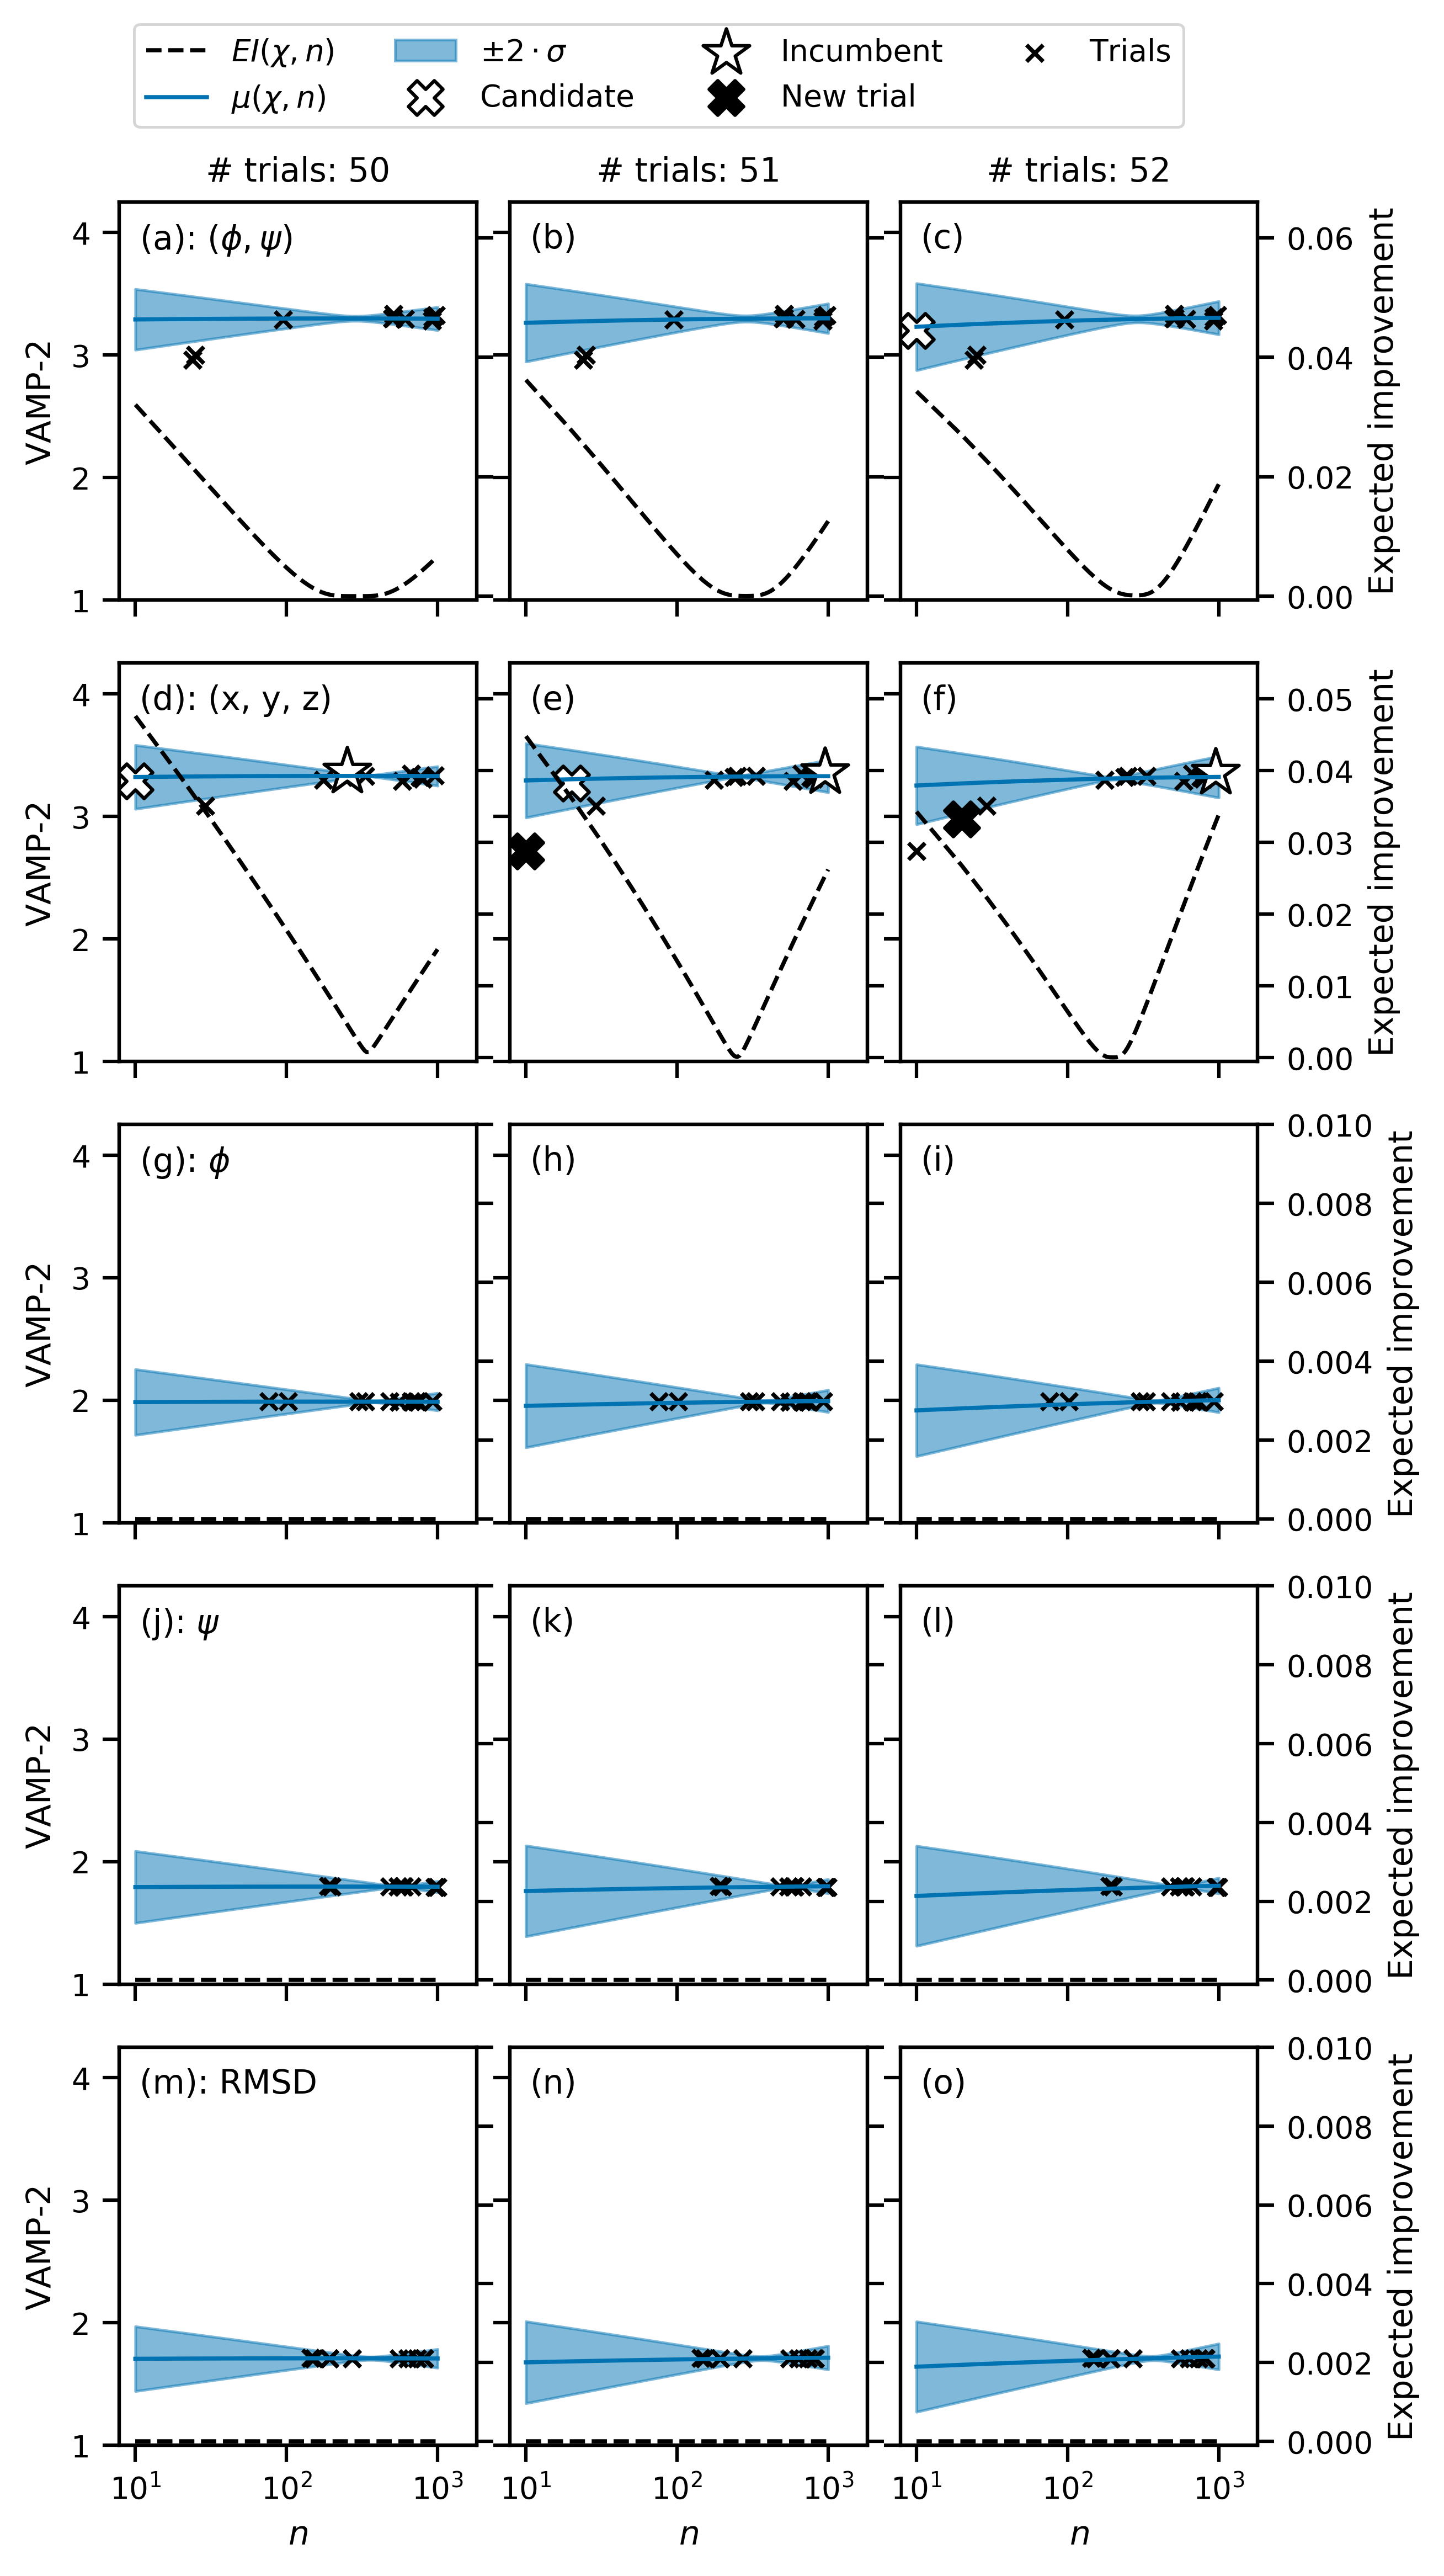
\includegraphics[height=0.8\textheight]{chapters/msm_optimization/figures/ala1_opt_explainer.png}
%     \label{fig:ala1_opt_expl}
% \end{figure}

\section{AADH}

\begin{table}
    \centering
    \caption{Model selection metrics for the response surface of AADH using all hyperparameter trials ($N=361$, except those for $\chi=$RMSD). The Mean Standardised Log Loss (MSLL) and Standardised Mean Square Error (SMSE) where calculated using 10 fold cross validation. Only those models which had both $\mathrm{MSLL}<0$ and $\mathrm{SMSE}<1$ were ranked. The total rank is calculated as rank of $\sqrt{R_{MSLL}^{2}+R_{SMSE}^2}$. Where the overall rank was tied, the first model appearing in the table was ranked higher. }
    \label{tab:aadh_rsm_metrics_all_data}
    \begin{tabularx}{1\textwidth}{|llllrr >{\raggedright\arraybackslash}X>{\raggedright\arraybackslash}X>{\raggedright\arraybackslash}X|}
    \hline
    $T(\tau)$ & $T(m)$ & $T(n)$ & Kernel & MSLL &   SMSE & Rank (MSLL) & Rank (SMSE) & Rank (Total)\\
    \hline\hline
    $I({\tau})$ & $I({m})$ & $I({n})$ & Exponential & -0.1298 & 0.3087 &       1.0 &       1.0 &  1.0 \\
                   &             & $\log({n})$ & Exponential &  0.0050 & 0.2964 &         - &         - &    - \\
                   & $\log({m})$ & $I({n})$ & Exponential &  0.0521 & 0.3118 &         - &         - &    - \\
                   &             & $\log({n})$ & Exponential &  0.5633 & 0.3815 &         - &         - &    - \\
    $\log({\tau})$ & $I({m})$ & $I({n})$ & Exponential &  0.1967 & 0.3436 &         - &         - &    - \\
                   &             & $\log({n})$ & Exponential &  0.4959 & 0.3231 &         - &         - &    - \\
                   & $\log({m})$ & $I({n})$ & Exponential &  0.5128 & 0.4365 &         - &         - &    - \\
                   &             & $\log({n})$ & Exponential &  1.0267 & 0.4201 &         - &         - &    - \\
    $I({\tau})$ & $I({m})$ & $I({n})$ & M32 &  1.5680 & 0.2893 &         - &         - &    - \\
                   &             & $\log({n})$ & M32 &  1.9193 & 0.2960 &         - &         - &    - \\
                   & $\log({m})$ & $I({n})$ & M32 &  3.1385 & 0.2775 &         - &         - &    - \\
                   &             & $\log({n})$ & M32 &  2.0358 & 0.2818 &         - &         - &    - \\
    $\log({\tau})$ & $I({m})$ & $I({n})$ & M32 &  6.9015 & 0.3203 &         - &         - &    - \\
                   &             & $\log({n})$ & M32 &  7.7182 & 0.3406 &         - &         - &    - \\
                   & $\log({m})$ & $I({n})$ & M32 &  7.9209 & 0.3257 &         - &         - &    - \\
                   &             & $\log({n})$ & M32 &  3.0002 & 0.3472 &         - &         - &    - \\
    $I({\tau})$ & $I({m})$ & $I({n})$ & M52 &  3.6517 & 0.3029 &         - &         - &    - \\
                   &             & $\log({n})$ & M52 &  3.8316 & 0.3090 &         - &         - &    - \\
                   & $\log({m})$ & $I({n})$ & M52 &  8.6574 & 0.2991 &         - &         - &    - \\
                   &             & $\log({n})$ & M52 &  3.7354 & 0.3238 &         - &         - &    - \\
    $\log({\tau})$ & $I({m})$ & $I({n})$ & M52 &  8.9207 & 0.3679 &         - &         - &    - \\
                   &             & $\log({n})$ & M52 & 11.8753 & 0.4064 &         - &         - &    - \\
                   & $\log({m})$ & $I({n})$ & M52 & 12.7637 & 0.3722 &         - &         - &    - \\
                   &             & $\log({n})$ & M52 & 13.6735 & 0.3475 &         - &         - &    - \\
    $I({\tau})$ & $I({m})$ & $I({n})$ & RBF &     inf &    inf &         - &         - &    - \\
                   &             & $\log({n})$ & RBF &  9.3618 & 0.3256 &         - &         - &    - \\
                   & $\log({m})$ & $I({n})$ & RBF &  5.9123 & 0.3022 &         - &         - &    - \\
                   &             & $\log({n})$ & RBF &     inf &    inf &         - &         - &    - \\
    $\log({\tau})$ & $I({m})$ & $I({n})$ & RBF & 17.4786 & 0.4551 &         - &         - &    - \\
                   &             & $\log({n})$ & RBF & 16.7568 & 0.3556 &         - &         - &    - \\
                   & $\log({m})$ & $I({n})$ & RBF & 16.7412 & 0.5026 &         - &         - &    - \\
                   &             & $\log({n})$ & RBF & 24.3199 & 0.4986 &         - &         - &    - \\
    \hline
    \end{tabularx}
\end{table}




\begin{table}
    \centering
    \caption{Model selection metrics for the response surface of an MSM of AADH, data subset 1, $N=100$, except those for $\chi=$RMSD). The Mean Standardised Log Loss (MSLL) and Standardised Mean Square Error (SMSE) where calculated using 10 fold cross validation. Only those models which had both $\mathrm{MSLL}<0$ and $\mathrm{SMSE}<1$ were ranked. The total rank is calculated as rank of $\sqrt{R_{MSLL}^{2}+R_{SMSE}^2}$. Where the overall rank was tied, the first model appearing in the table was ranked higher. }
    \label{tab:aadh_rsm_metrics_iter_1}
    \begin{tabularx}{1\textwidth}{|llllrr >{\raggedright\arraybackslash}X>{\raggedright\arraybackslash}X>{\raggedright\arraybackslash}X|}
    \hline
    $T(\tau)$ & $T(m)$ & $T(n)$ & Kernel & MSLL &   SMSE & Rank (MSLL) & Rank (SMSE) & Rank (Total)\\
    \hline\hline
    $I({\tau})$ & $I({m})$ & $I({n})$ & Exponential & -0.3928 & 0.3412 &        10.0 &        14.0 &         13.0 \\
               &             & $\log({n})$ & Exponential & -0.2456 & 0.3443 &        15.0 &        15.0 &         16.0 \\
               & $\log({m})$ & $I({n})$ & Exponential & -0.6484 & 0.3169 &         6.0 &        12.0 &          7.0 \\
               &             & $\log({n})$ & Exponential & -0.5585 & 0.3487 &         7.0 &        17.0 &         14.0 \\
    $\log({\tau})$ & $I({m})$ & $I({n})$ & Exponential &  0.0598 & 0.3483 &           - &           - &            - \\
                   &             & $\log({n})$ & Exponential & -0.2195 & 0.3450 &        16.0 &        16.0 &         17.0 \\
                   & $\log({m})$ & $I({n})$ & Exponential & -0.3524 & 0.3084 &        13.0 &         9.0 &         10.0 \\
                   &             & $\log({n})$ & Exponential & -0.3944 & 0.3379 &         9.0 &        13.0 &         11.0 \\
    $I({\tau})$ & $I({m})$ & $I({n})$ & M32 & -0.3807 & 0.3167 &        12.0 &        11.0 &         12.0 \\
                   &             & $\log({n})$ & M32 & -0.2744 & 0.3053 &        14.0 &         7.0 &          9.0 \\
                   & $\log({m})$ & $I({n})$ & M32 & -0.8769 & 0.2779 &         1.0 &         4.0 &          3.0 \\
                   &             & $\log({n})$ & M32 & -0.7438 & 0.2785 &         5.0 &         5.0 &          5.0 \\
    $\log({\tau})$ & $I({m})$ & $I({n})$ & M32 &  0.3415 & 0.3721 &           - &           - &            - \\
                   &             & $\log({n})$ & M32 & -0.2023 & 0.3892 &        17.0 &        18.0 &         18.0 \\
                   & $\log({m})$ & $I({n})$ & M32 & -0.4758 & 0.3033 &         8.0 &         6.0 &          6.0 \\
                   &             & $\log({n})$ & M32 & -0.3892 & 0.3086 &        11.0 &        10.0 &          8.0 \\
    $I({\tau})$ & $I({m})$ & $I({n})$ & M52 &  0.3362 & 0.3149 &           - &           - &            - \\
                   &             & $\log({n})$ & M52 &  0.9964 & 0.2712 &           - &           - &            - \\
                   & $\log({m})$ & $I({n})$ & M52 & -0.8713 & 0.2685 &         2.0 &         2.0 &          1.0 \\
                   &             & $\log({n})$ & M52 & -0.7508 & 0.2700 &         4.0 &         3.0 &          4.0 \\
    $\log({\tau})$ & $I({m})$ & $I({n})$ & M52 &  6.4201 & 0.3503 &           - &           - &            - \\
                   &             & $\log({n})$ & M52 &  5.7695 & 0.3250 &           - &           - &            - \\
                   & $\log({m})$ & $I({n})$ & M52 &  3.9718 & 0.3153 &           - &           - &            - \\
                   &             & $\log({n})$ & M52 &     inf &    inf &           - &           - &            - \\
    $I({\tau})$ & $I({m})$ & $I({n})$ & RBF & -0.1677 & 0.3074 &        18.0 &         8.0 &         15.0 \\
                   &             & $\log({n})$ & RBF &  1.3068 & 0.2747 &           - &           - &            - \\
                   & $\log({m})$ & $I({n})$ & RBF & -0.7884 & 0.2675 &         3.0 &         1.0 &          2.0 \\
                   &             & $\log({n})$ & RBF &     inf &    inf &           - &           - &            - \\
    $\log({\tau})$ & $I({m})$ & $I({n})$ & RBF &  6.8541 & 0.3472 &           - &           - &            - \\
                   &             & $\log({n})$ & RBF &  6.2984 & 0.3074 &           - &           - &            - \\
                   & $\log({m})$ & $I({n})$ & RBF &  4.8742 & 0.4157 &           - &           - &            - \\
                   &             & $\log({n})$ & RBF &  7.6739 & 0.5531 &           - &           - &            - \\
    \hline
    \end{tabularx}
\end{table}

\begin{table}
    \centering
    \caption{Model selection metrics for the response surface of an MSM of AADH, data subset 2, $N=100$, except those for $\chi=$RMSD). The Mean Standardised Log Loss (MSLL) and Standardised Mean Square Error (SMSE) where calculated using 10 fold cross validation. Only those models which had both $\mathrm{MSLL}<0$ and $\mathrm{SMSE}<1$ were ranked. The total rank is calculated as rank of $\sqrt{R_{MSLL}^{2}+R_{SMSE}^2}$. Where the overall rank was tied, the first model appearing in the table was ranked higher. }
    \label{tab:aadh_rsm_metrics_iter_2}
    \begin{tabularx}{1\textwidth}{|llllrr >{\raggedright\arraybackslash}X>{\raggedright\arraybackslash}X>{\raggedright\arraybackslash}X|}
    \hline
    $T(\tau)$ & $T(m)$ & $T(n)$ & Kernel & MSLL &   SMSE & Rank (MSLL) & Rank (SMSE) & Rank (Total)\\
    \hline\hline
    $I({\tau})$ & $I({m})$ & $I({n})$ & Exponential & -0.3293 & 0.4262 &        13.0 &         9.0 &         11.0 \\
                   &             & $\log({n})$ & Exponential & -0.5222 & 0.4330 &         6.0 &        13.0 &          8.0 \\
                   & $\log({m})$ & $I({n})$ & Exponential & -0.6612 & 0.3890 &         1.0 &         2.0 &          1.0 \\
                   &             & $\log({n})$ & Exponential & -0.5843 & 0.4170 &         3.0 &         5.0 &          3.0 \\
    $\log({\tau})$ & $I({m})$ & $I({n})$ & Exponential & -0.3737 & 0.4590 &        11.0 &        15.0 &         15.0 \\
                   &             & $\log({n})$ & Exponential & -0.4162 & 0.4445 &         8.0 &        14.0 &         12.0 \\
                   & $\log({m})$ & $I({n})$ & Exponential & -0.3702 & 0.4281 &        12.0 &        10.0 &         10.0 \\
                   &             & $\log({n})$ & Exponential & -0.6242 & 0.4169 &         2.0 &         4.0 &          2.0 \\
    $I({\tau})$ & $I({m})$ & $I({n})$ & M32 & -0.5737 & 0.4218 &         4.0 &         7.0 &          5.0 \\
                   &             & $\log({n})$ & M32 &  0.1639 & 0.4432 &           - &           - &            - \\
                   & $\log({m})$ & $I({n})$ & M32 & -0.5479 & 0.4282 &         5.0 &        11.0 &          7.0 \\
                   &             & $\log({n})$ & M32 & -0.4595 & 0.3844 &         7.0 &         1.0 &          4.0 \\
    $\log({\tau})$ & $I({m})$ & $I({n})$ & M32 & -0.4077 & 0.4301 &         9.0 &        12.0 &          9.0 \\
                   &             & $\log({n})$ & M32 &     inf &    inf &           - &           - &            - \\
                   & $\log({m})$ & $I({n})$ & M32 &  1.0248 & 0.4609 &           - &           - &            - \\
                   &             & $\log({n})$ & M32 & -0.3902 & 0.3942 &        10.0 &         3.0 &          6.0 \\
    $I({\tau})$ & $I({m})$ & $I({n})$ & M52 &  1.3964 & 0.4033 &           - &           - &            - \\
                   &             & $\log({n})$ & M52 &  0.3681 & 0.4475 &           - &           - &            - \\
                   & $\log({m})$ & $I({n})$ & M52 & -0.1968 & 0.4237 &        14.0 &         8.0 &         13.0 \\
                   &             & $\log({n})$ & M52 &  2.3201 & 0.4400 &           - &           - &            - \\
    $\log({\tau})$ & $I({m})$ & $I({n})$ & M52 &  3.2132 & 0.4125 &           - &           - &            - \\
                   &             & $\log({n})$ & M52 &  0.5430 & 0.4473 &           - &           - &            - \\
                   & $\log({m})$ & $I({n})$ & M52 &  1.6455 & 0.4679 &           - &           - &            - \\
                   &             & $\log({n})$ & M52 &  0.7421 & 0.4378 &           - &           - &            - \\
    $I({\tau})$ & $I({m})$ & $I({n})$ & RBF &  2.3960 & 0.4042 &           - &           - &            - \\
                   &             & $\log({n})$ & RBF &  1.3825 & 0.4372 &           - &           - &            - \\
                   & $\log({m})$ & $I({n})$ & RBF & -0.1688 & 0.4197 &        15.0 &         6.0 &         14.0 \\
                   &             & $\log({n})$ & RBF &  3.8725 & 0.4652 &           - &           - &            - \\
    $\log({\tau})$ & $I({m})$ & $I({n})$ & RBF &  4.1994 & 0.4244 &           - &           - &            - \\
                   &             & $\log({n})$ & RBF &  2.3169 & 0.4305 &           - &           - &            - \\
                   & $\log({m})$ & $I({n})$ & RBF &  1.7600 & 0.4764 &           - &           - &            - \\
                   &             & $\log({n})$ & RBF &  1.6457 & 0.4517 &           - &           - &            - \\
    \hline
    \end{tabularx}
\end{table}


\begin{table}
    \centering
    \caption{Model selection metrics for the response surface of an MSM of AADH, data subset 3, $N=100$, except those for $\chi=$RMSD). The Mean Standardised Log Loss (MSLL) and Standardised Mean Square Error (SMSE) where calculated using 10 fold cross validation. Only those models which had both $\mathrm{MSLL}<0$ and $\mathrm{SMSE}<1$ were ranked. The total rank is calculated as rank of $\sqrt{R_{MSLL}^{2}+R_{SMSE}^2}$. Where the overall rank was tied, the first model appearing in the table was ranked higher. }
    \label{tab:aadh_rsm_metrics_iter_3}
    \begin{tabularx}{1\textwidth}{|llllrr >{\raggedright\arraybackslash}X>{\raggedright\arraybackslash}X>{\raggedright\arraybackslash}X|}
    \hline
    $T(\tau)$ & $T(m)$ & $T(n)$ & Kernel & MSLL &   SMSE & Rank (MSLL) & Rank (SMSE) & Rank (Total)\\
    \hline\hline
    $I({\tau})$ & $I({m})$ & $I({n})$ & Exponential & -0.4461 & 0.5415 &        14.0 &        15.0 &         13.0 \\
                   &             & $\log({n})$ & Exponential & -0.4350 & 0.5234 &        15.0 &         9.0 &         10.0 \\
                   & $\log({m})$ & $I({n})$ & Exponential & -0.6123 & 0.5074 &         6.0 &         5.0 &          3.0 \\
                   &             & $\log({n})$ & Exponential & -0.5378 & 0.5145 &         9.0 &         7.0 &          5.0 \\
    $\log({\tau})$ & $I({m})$ & $I({n})$ & Exponential & -0.3138 & 0.6006 &        21.0 &        25.0 &         24.0 \\
                   &             & $\log({n})$ & Exponential & -0.3559 & 0.5626 &        20.0 &        21.0 &         22.0 \\
                   & $\log({m})$ & $I({n})$ & Exponential & -0.4587 & 0.5449 &        13.0 &        17.0 &         14.0 \\
                   &             & $\log({n})$ & Exponential & -0.4276 & 0.5472 &        18.0 &        18.0 &         20.0 \\
    $I({\tau})$ & $I({m})$ & $I({n})$ & M32 & -0.6003 & 0.5234 &         7.0 &         8.0 &          4.0 \\
                   &             & $\log({n})$ & M32 & -0.6400 & 0.5376 &         5.0 &        12.0 &          8.0 \\
                   & $\log({m})$ & $I({n})$ & M32 & -0.8017 & 0.4885 &         2.0 &         1.0 &          1.0 \\
                   &             & $\log({n})$ & M32 & -0.8921 & 0.4892 &         1.0 &         2.0 &          2.0 \\
    $\log({\tau})$ & $I({m})$ & $I({n})$ & M32 & -0.1904 & 0.5933 &        24.0 &        24.0 &         25.0 \\
                   &             & $\log({n})$ & M32 & -0.4898 & 0.5711 &        11.0 &        22.0 &         18.0 \\
                   & $\log({m})$ & $I({n})$ & M32 & -0.4295 & 0.5379 &        17.0 &        13.0 &         15.0 \\
                   &             & $\log({n})$ & M32 & -0.6808 & 0.5350 &         4.0 &        11.0 &          6.0 \\
    $I({\tau})$ & $I({m})$ & $I({n})$ & M52 & -0.4328 & 0.5482 &        16.0 &        19.0 &         19.0 \\
                   &             & $\log({n})$ & M52 & -0.5392 & 0.5262 &         8.0 &        10.0 &          7.0 \\
                   & $\log({m})$ & $I({n})$ & M52 & -0.7498 & 0.5506 &         3.0 &        20.0 &         12.0 \\
                   &             & $\log({n})$ & M52 & -0.2438 & 0.5141 &        22.0 &         6.0 &         16.0 \\
    $\log({\tau})$ & $I({m})$ & $I({n})$ & M52 &  0.4797 & 0.6354 &           - &           - &            - \\
                   &             & $\log({n})$ & M52 & -0.3604 & 0.6100 &        19.0 &        26.0 &         23.0 \\
                   & $\log({m})$ & $I({n})$ & M52 & -0.1492 & 0.5818 &        25.0 &        23.0 &         26.0 \\
                   &             & $\log({n})$ & M52 &  0.1426 & 0.5263 &           - &           - &            - \\
    $I({\tau})$ & $I({m})$ & $I({n})$ & RBF & -0.5234 & 0.5412 &        10.0 &        14.0 &          9.0 \\
                   &             & $\log({n})$ & RBF & -0.4854 & 0.5436 &        12.0 &        16.0 &         11.0 \\
                   & $\log({m})$ & $I({n})$ & RBF &     inf &    inf &           - &           - &            - \\
                   &             & $\log({n})$ & RBF & -0.1291 & 0.5002 &        26.0 &         3.0 &         21.0 \\
    $\log({\tau})$ & $I({m})$ & $I({n})$ & RBF &  1.5339 & 0.5471 &           - &           - &            - \\
                   &             & $\log({n})$ & RBF & -0.0794 & 0.6378 &        27.0 &        27.0 &         27.0 \\
                   & $\log({m})$ & $I({n})$ & RBF & -0.2000 & 0.5068 &        23.0 &         4.0 &         17.0 \\
                   &             & $\log({n})$ & RBF &  0.1399 & 0.4935 &           - &           - &            - \\
    \hline
    \end{tabularx}
\end{table}


\begin{table}
    \centering
    \caption{Model selection metrics for the response surface of an MSM of AADH, data subset 4, $N=100$, except those for $\chi=$RMSD). The Mean Standardised Log Loss (MSLL) and Standardised Mean Square Error (SMSE) where calculated using 10 fold cross validation. Only those models which had both $\mathrm{MSLL}<0$ and $\mathrm{SMSE}<1$ were ranked. The total rank is calculated as rank of $\sqrt{R_{MSLL}^{2}+R_{SMSE}^2}$. Where the overall rank was tied, the first model appearing in the table was ranked higher. }
    \label{tab:aadh_rsm_metrics_iter_4}
    \begin{tabularx}{1\textwidth}{|llllrr >{\raggedright\arraybackslash}X>{\raggedright\arraybackslash}X>{\raggedright\arraybackslash}X|}
    \hline
    $T(\tau)$ & $T(m)$ & $T(n)$ & Kernel & MSLL &   SMSE & Rank (MSLL) & Rank (SMSE) & Rank (Total)\\
    \hline\hline
    $I({\tau})$ & $I({m})$ & $I({n})$ & Exponential & -0.7560 & 0.2203 &         8.0 &        16.0 &         16.0 \\
                   &             & $\log({n})$ & Exponential & -0.7875 & 0.2181 &         7.0 &        15.0 &         15.0 \\
                   & $\log({m})$ & $I({n})$ & Exponential & -0.9947 & 0.1510 &         3.0 &        10.0 &          4.0 \\
                   &             & $\log({n})$ & Exponential & -0.9846 & 0.1449 &         4.0 &         9.0 &          3.0 \\
    $\log({\tau})$ & $I({m})$ & $I({n})$ & Exponential & -0.8015 & 0.2132 &         6.0 &        14.0 &         12.0 \\
                   &             & $\log({n})$ & Exponential & -0.8752 & 0.1825 &         5.0 &        13.0 &          7.0 \\
                   & $\log({m})$ & $I({n})$ & Exponential & -1.0363 & 0.1442 &         1.0 &         8.0 &          2.0 \\
                   &             & $\log({n})$ & Exponential & -1.0279 & 0.1327 &         2.0 &         6.0 &          1.0 \\
    $I({\tau})$ & $I({m})$ & $I({n})$ & M32 &     inf &    inf &           - &           - &            - \\
                   &             & $\log({n})$ & M32 & -0.5648 & 0.1809 &        10.0 &        12.0 &         13.0 \\
                   & $\log({m})$ & $I({n})$ & M32 & -0.4921 & 6.5461 &           - &           - &            - \\
                   &             & $\log({n})$ & M32 & -0.5509 & 0.1001 &        11.0 &         1.0 &          5.0 \\
    $\log({\tau})$ & $I({m})$ & $I({n})$ & M32 & 17.1108 & 4.4912 &           - &           - &            - \\
                   &             & $\log({n})$ & M32 & -0.2896 & 0.1322 &        13.0 &         5.0 &          8.0 \\
                   & $\log({m})$ & $I({n})$ & M32 &  0.8341 & 6.6805 &           - &           - &            - \\
                   &             & $\log({n})$ & M32 & -0.6497 & 0.1530 &         9.0 &        11.0 &          9.0 \\
    $I({\tau})$ & $I({m})$ & $I({n})$ & M52 &  0.0998 & 0.1507 &           - &           - &            - \\
                   &             & $\log({n})$ & M52 &  0.2457 & 0.1419 &           - &           - &            - \\
                   & $\log({m})$ & $I({n})$ & M52 & -0.2353 & 0.1103 &        15.0 &         2.0 &         11.0 \\
                   &             & $\log({n})$ & M52 &  0.1854 & 0.0885 &           - &           - &            - \\
    $\log({\tau})$ & $I({m})$ & $I({n})$ & M52 &  0.1737 & 0.1471 &           - &           - &            - \\
                   &             & $\log({n})$ & M52 &  0.1300 & 0.1468 &           - &           - &            - \\
                   & $\log({m})$ & $I({n})$ & M52 & -0.2515 & 0.1228 &        14.0 &         4.0 &         10.0 \\
                   &             & $\log({n})$ & M52 & -0.3690 & 0.1335 &        12.0 &         7.0 &          6.0 \\
    $I({\tau})$ & $I({m})$ & $I({n})$ & RBF &  0.4745 & 0.1570 &           - &           - &            - \\
                   &             & $\log({n})$ & RBF &  0.3424 & 0.1426 &           - &           - &            - \\
                   & $\log({m})$ & $I({n})$ & RBF & -0.0644 & 0.1120 &        16.0 &         3.0 &         14.0 \\
                   &             & $\log({n})$ & RBF &  0.6375 & 0.0887 &           - &           - &            - \\
    $\log({\tau})$ & $I({m})$ & $I({n})$ & RBF &  0.5639 & 0.1596 &           - &           - &            - \\
                   &             & $\log({n})$ & RBF &  0.9161 & 0.1642 &           - &           - &            - \\
                   & $\log({m})$ & $I({n})$ & RBF &  0.2483 & 0.1132 &           - &           - &            - \\
                   &             & $\log({n})$ & RBF &  0.1566 & 0.1366 &           - &           - &            - \\
    \hline
    \end{tabularx}
\end{table}

\begin{table}
    \centering
    \caption{Model selection metrics for the response surface of an MSM of AADH, data subset 5, $N=100$, except those for $\chi=$RMSD). The Mean Standardised Log Loss (MSLL) and Standardised Mean Square Error (SMSE) where calculated using 10 fold cross validation. Only those models which had both $\mathrm{MSLL}<0$ and $\mathrm{SMSE}<1$ were ranked. The total rank is calculated as rank of $\sqrt{R_{MSLL}^{2}+R_{SMSE}^2}$. Where the overall rank was tied, the first model appearing in the table was ranked higher. }
    \label{tab:aadh_rsm_metrics_iter_5}
    \begin{tabularx}{1\textwidth}{|llllrr >{\raggedright\arraybackslash}X>{\raggedright\arraybackslash}X>{\raggedright\arraybackslash}X|}
    \hline
    $T(\tau)$ & $T(m)$ & $T(n)$ & Kernel & MSLL &   SMSE & Rank (MSLL) & Rank (SMSE) & Rank (Total)\\
    \hline\hline
    $I({\tau})$ & $I({m})$ & $I({n})$ & Exponential & -0.4560 & 0.3075 &         4.0 &        16.0 &         11.0 \\
                   &             & $\log({n})$ & Exponential & -0.3903 & 0.3240 &         8.0 &        19.0 &         18.0 \\
                   & $\log({m})$ & $I({n})$ & Exponential & -0.2797 & 0.3010 &        13.0 &        15.0 &         15.0 \\
                   &             & $\log({n})$ & Exponential & -0.4260 & 0.2957 &         5.0 &        14.0 &          8.0 \\
    $\log({\tau})$ & $I({m})$ & $I({n})$ & Exponential & -0.3979 & 0.3182 &         7.0 &        18.0 &         12.0 \\
                   &             & $\log({n})$ & Exponential & -0.3533 & 0.3126 &        10.0 &        17.0 &         13.0 \\
                   & $\log({m})$ & $I({n})$ & Exponential & -0.2961 & 0.2828 &        12.0 &        11.0 &         10.0 \\
                   &             & $\log({n})$ & Exponential & -0.1504 & 0.2821 &        17.0 &        10.0 &         14.0 \\
    $I({\tau})$ & $I({m})$ & $I({n})$ & M32 & -0.2251 & 0.2832 &        16.0 &        12.0 &         17.0 \\
                   &             & $\log({n})$ & M32 & -0.4864 & 0.2769 &         3.0 &         9.0 &          4.0 \\
                   & $\log({m})$ & $I({n})$ & M32 & -0.3340 & 0.2395 &        11.0 &         2.0 &          5.0 \\
                   &             & $\log({n})$ & M32 & -0.2605 & 0.2408 &        14.0 &         4.0 &          7.0 \\
    $\log({\tau})$ & $I({m})$ & $I({n})$ & M32 &  0.6857 & 0.2878 &           - &           - &            - \\
                   &             & $\log({n})$ & M32 &  0.6788 & 0.2833 &           - &           - &            - \\
                   & $\log({m})$ & $I({n})$ & M32 & -0.0028 & 0.2589 &        19.0 &         6.0 &         16.0 \\
                   &             & $\log({n})$ & M32 &  2.5955 & 0.2787 &           - &           - &            - \\
    $I({\tau})$ & $I({m})$ & $I({n})$ & M52 & -0.0040 & 0.2865 &        18.0 &        13.0 &         19.0 \\
                   &             & $\log({n})$ & M52 & -0.3897 & 0.2747 &         9.0 &         8.0 &          6.0 \\
                   & $\log({m})$ & $I({n})$ & M52 & -0.7173 & 0.2285 &         1.0 &         1.0 &          1.0 \\
                   &             & $\log({n})$ & M52 & -0.6388 & 0.2406 &         2.0 &         3.0 &          2.0 \\
    $\log({\tau})$ & $I({m})$ & $I({n})$ & M52 &  0.3359 & 0.2922 &           - &           - &            - \\
                   &             & $\log({n})$ & M52 &  1.9673 & 0.2817 &           - &           - &            - \\
                   & $\log({m})$ & $I({n})$ & M52 & -0.2367 & 0.2533 &        15.0 &         5.0 &          9.0 \\
                   &             & $\log({n})$ & M52 &  2.4714 & 0.2870 &           - &           - &            - \\
    $I({\tau})$ & $I({m})$ & $I({n})$ & RBF &  2.5656 & 0.2672 &           - &           - &            - \\
                   &             & $\log({n})$ & RBF & -0.4234 & 0.2669 &         6.0 &         7.0 &          3.0 \\
                   & $\log({m})$ & $I({n})$ & RBF &  1.0865 & 0.2423 &           - &           - &            - \\
                   &             & $\log({n})$ & RBF &  0.2375 & 0.2507 &           - &           - &            - \\
    $\log({\tau})$ & $I({m})$ & $I({n})$ & RBF &  3.6181 & 0.2821 &           - &           - &            - \\
                   &             & $\log({n})$ & RBF &  1.8240 & 0.2790 &           - &           - &            - \\
                   & $\log({m})$ & $I({n})$ & RBF &  0.3803 & 0.2535 &           - &           - &            - \\
                   &             & $\log({n})$ & RBF &  6.8263 & 0.2731 &           - &           - &            - \\
    \hline
    \end{tabularx}
\end{table}

\chapter{Metastable state selection for hidden Markov models}\label{app:hmm}

\section{Prinz potential}
 The Prinz potential is given by: 
\begin{equation}\label{eqn:prinz_pot}
       V(x) = 4\left(x^8 + 0.8 \exp{\left(-80 x^2\right)} + 0.2 \exp{\left(-80 (x-0.5)^2\right)} + 0.5\exp{\left(-40 (x+0.5)^2\right)}\right).
\end{equation}
Exact eigenvalues and trajectories of simulated Brownian motion were calculated using code from MSMBuilder \cite{beauchampMSMBuilder2ModelingConformational2011} version 3.9.0.  The first $7$ relaxation processes are given in table \ref{tab:prinz_its_exact}. 
\begin{table}
    \centering
    \mycaption{Relaxation timescales of the Prinz potential. All values are given in units of the time step $\Delta t = 0.001$}
    \begin{tabular}{|c|c|}
        \hline
        Process, $i$ & $t_i$ \\
        \hline\hline
         2 & 844.4 \\
         3 & 125.5 \\
         4 & 64.3 \\
         5 & 11.9 \\
         6 & 10.3 \\
         7 & 7.3 \\
         8 & 6.7 \\
         \hline
    \end{tabular}
    \label{tab:prinz_its_exact}
\end{table}

100 trajectories of Brownian dynamics were simulated by the following stochastic differential equation: 

\begin{equation}\label{eqn:prinz_dynamics}
    \frac{\mathrm{d}x_t}{\mathrm{d}t} = -\frac{\mathrm{d}V(x)}{\mathrm{d}x} + \sqrt{2D} * R(t)
\end{equation}

with $D = 1000$, and $R\sim \mathcal{N}(0, 1)$, $\mathrm{Cov}\left[R(t), R(t^{\prime})\right]=\delta_{t, t^{\prime}}$. The time-step used was $\Delta t = 0.001$.  Each trajectory was initiated from a random draw of the stationary distribution and was twice the longest relaxation process timescale, i.e. $2\times 844=1688$ time-steps long. The trajectories were clustered into $n = \left\lfloor\sqrt{100\times 1688}\right\rfloor =410$ discrete states using k-means clustering \cite{friedman2001elements}. This number of states was based on the heuristic described in \cite{husicWardClusteringImproves2017a}.


\chapter{AADH}\label{app:aadh}
\section{Molecular dynamics}

\begin{figure}[p]
    \centering
    \mycaption{LOW RESOLUTION! RMSD of the $\alpha$-Carbon atoms of AADH relative to the crystal structure. Each panel is a single trajectory, blue lines are the RMSD, black horizontal lines are the \SI{2.5}{\percent} and \SI{97.5}{\percent} quantiles (\SI{4.5}{\angstrom} and \SI{6.4}{\angstrom}, respectively) taken across all trajectories.}
    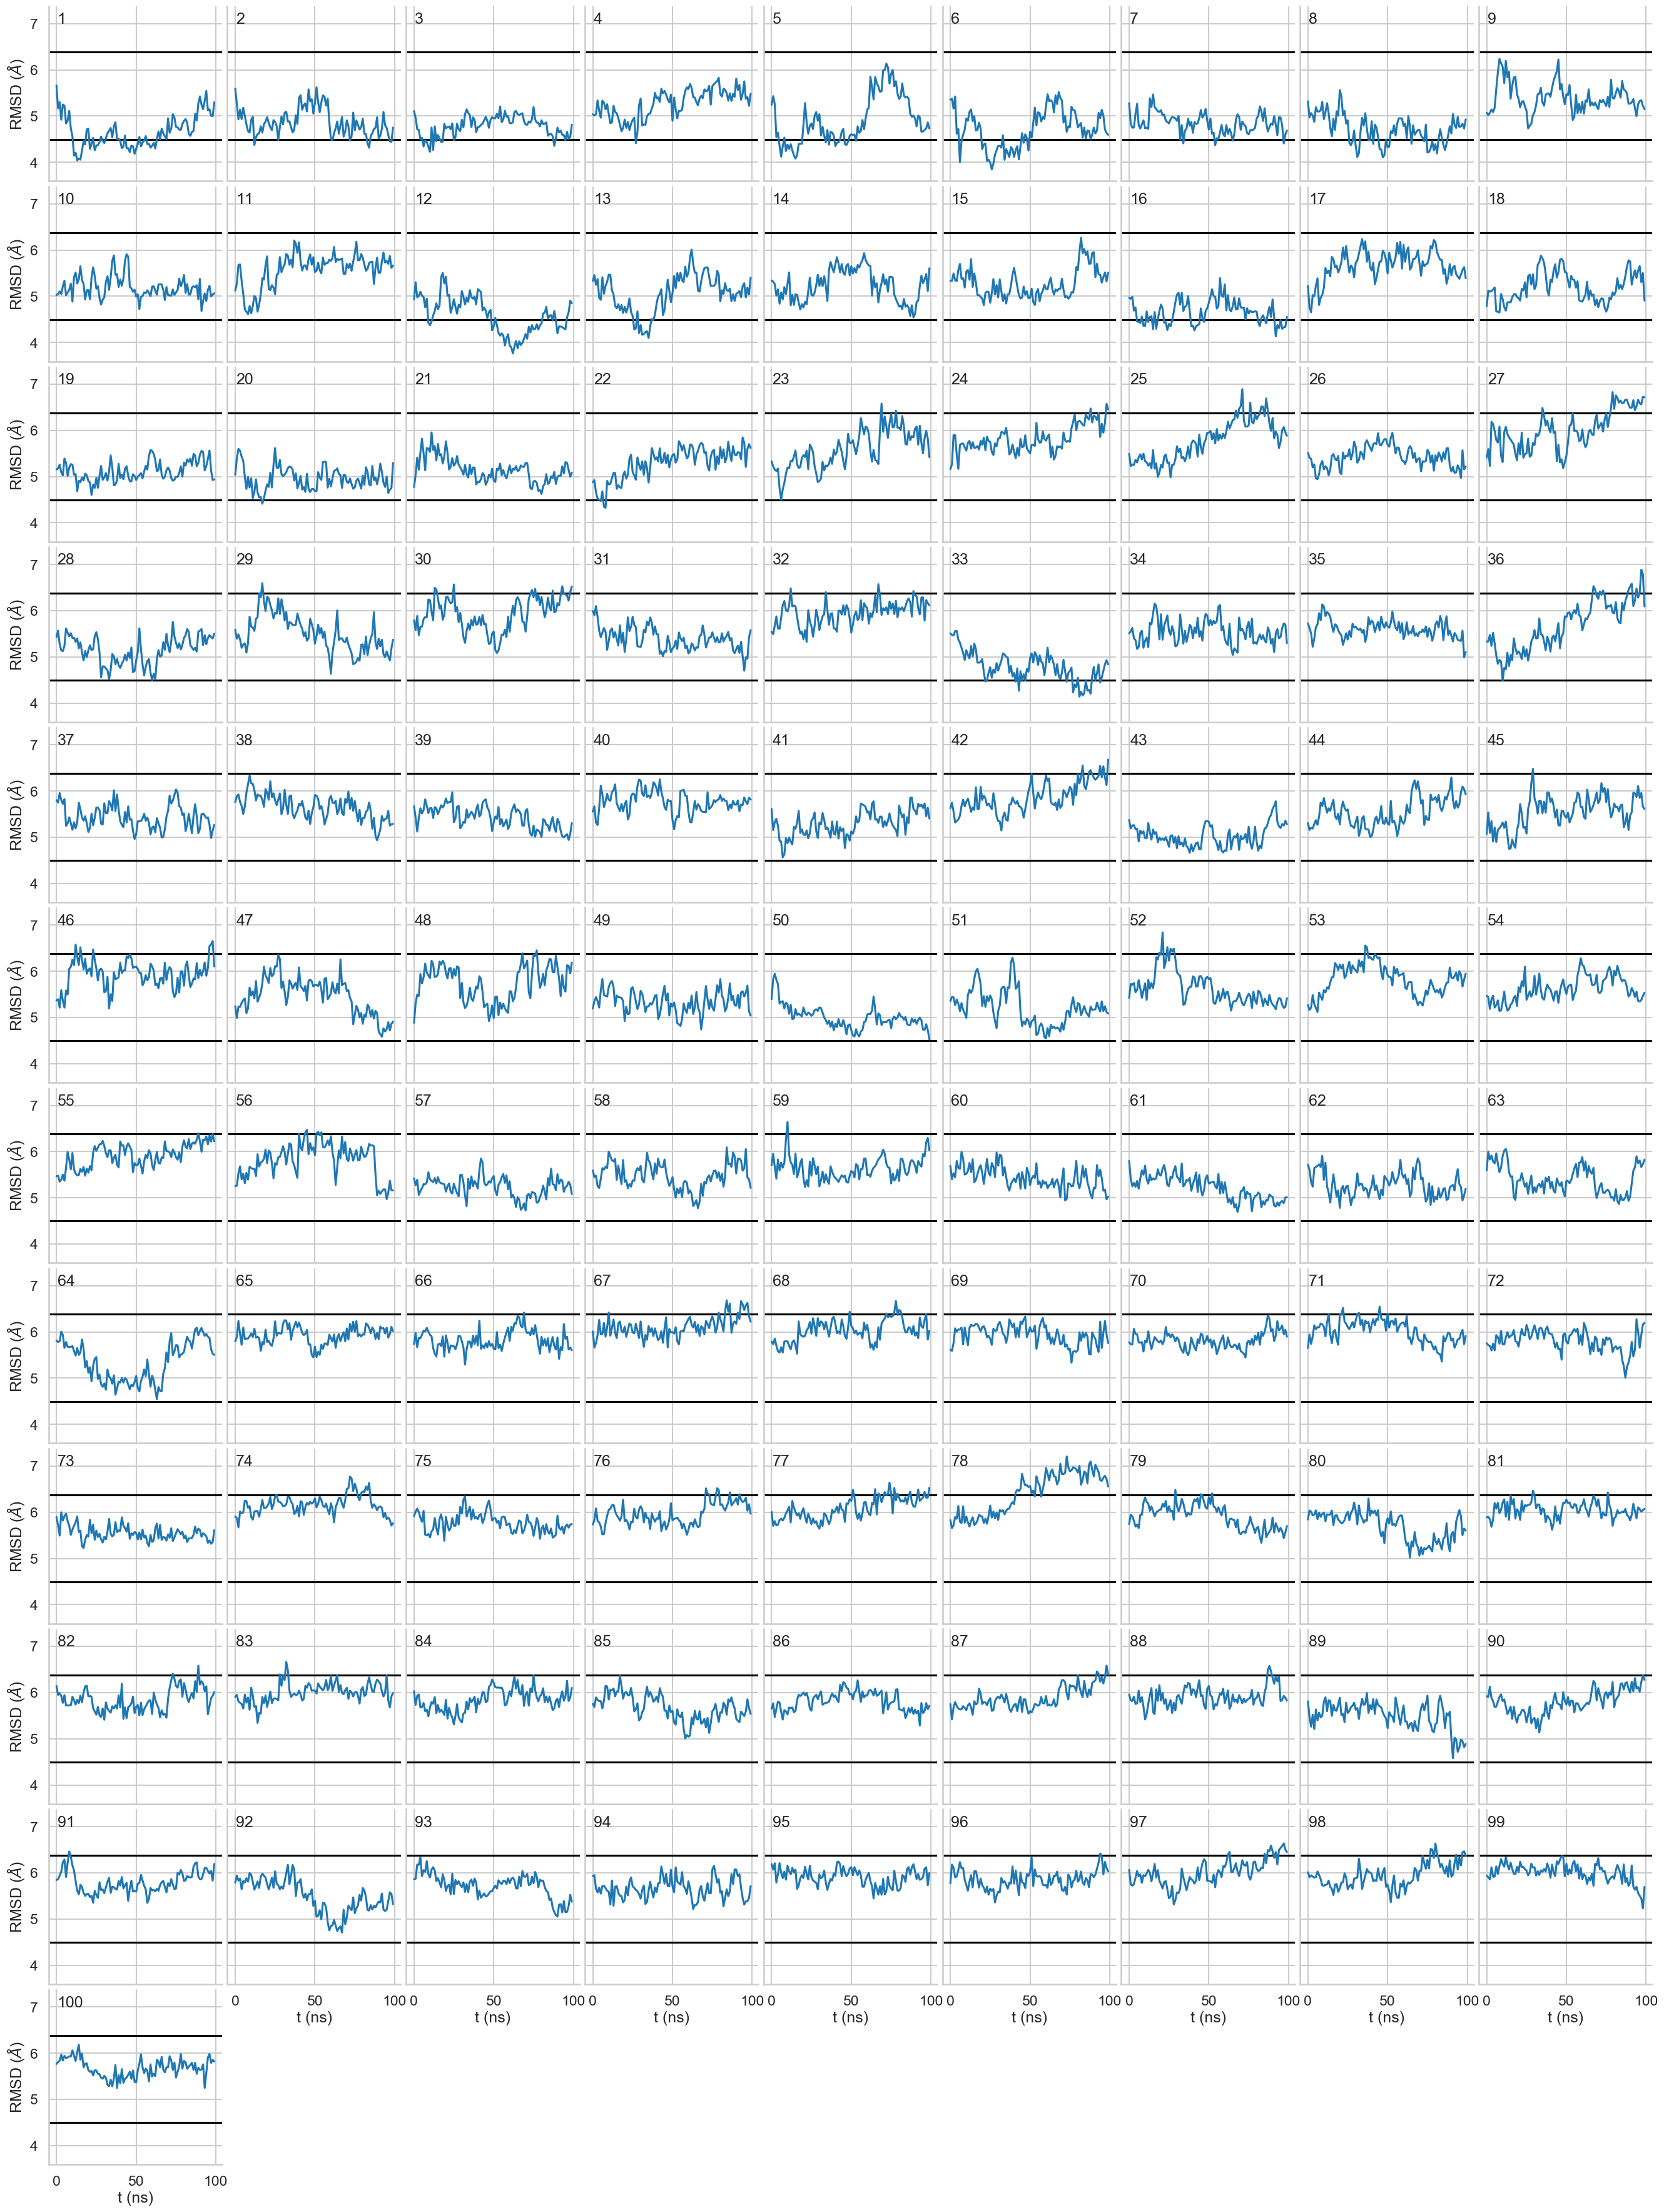
\includegraphics[width=0.9\textwidth]{chapters/aadh/figures/rmsd_backbone_ca.png}
    \label{fig:rmsd_ca}
\end{figure}

\begin{figure}
    \centering
    \mycaption{Secondary structure composition of trajectories $24, 27, 30, 42, 78, 87$ and $97$ as a function of time. The number of residues in each simplified secondary structure class \cite{kabschDictionaryProteinSecondary1983} are shown: `H' (green) refers to alpha helix, 3- and 5-helices; `E' (orange) refers to residues in beta-bridges or  beta ladder; `C' (blue) refers to turns, bends and all irregular elements.}
    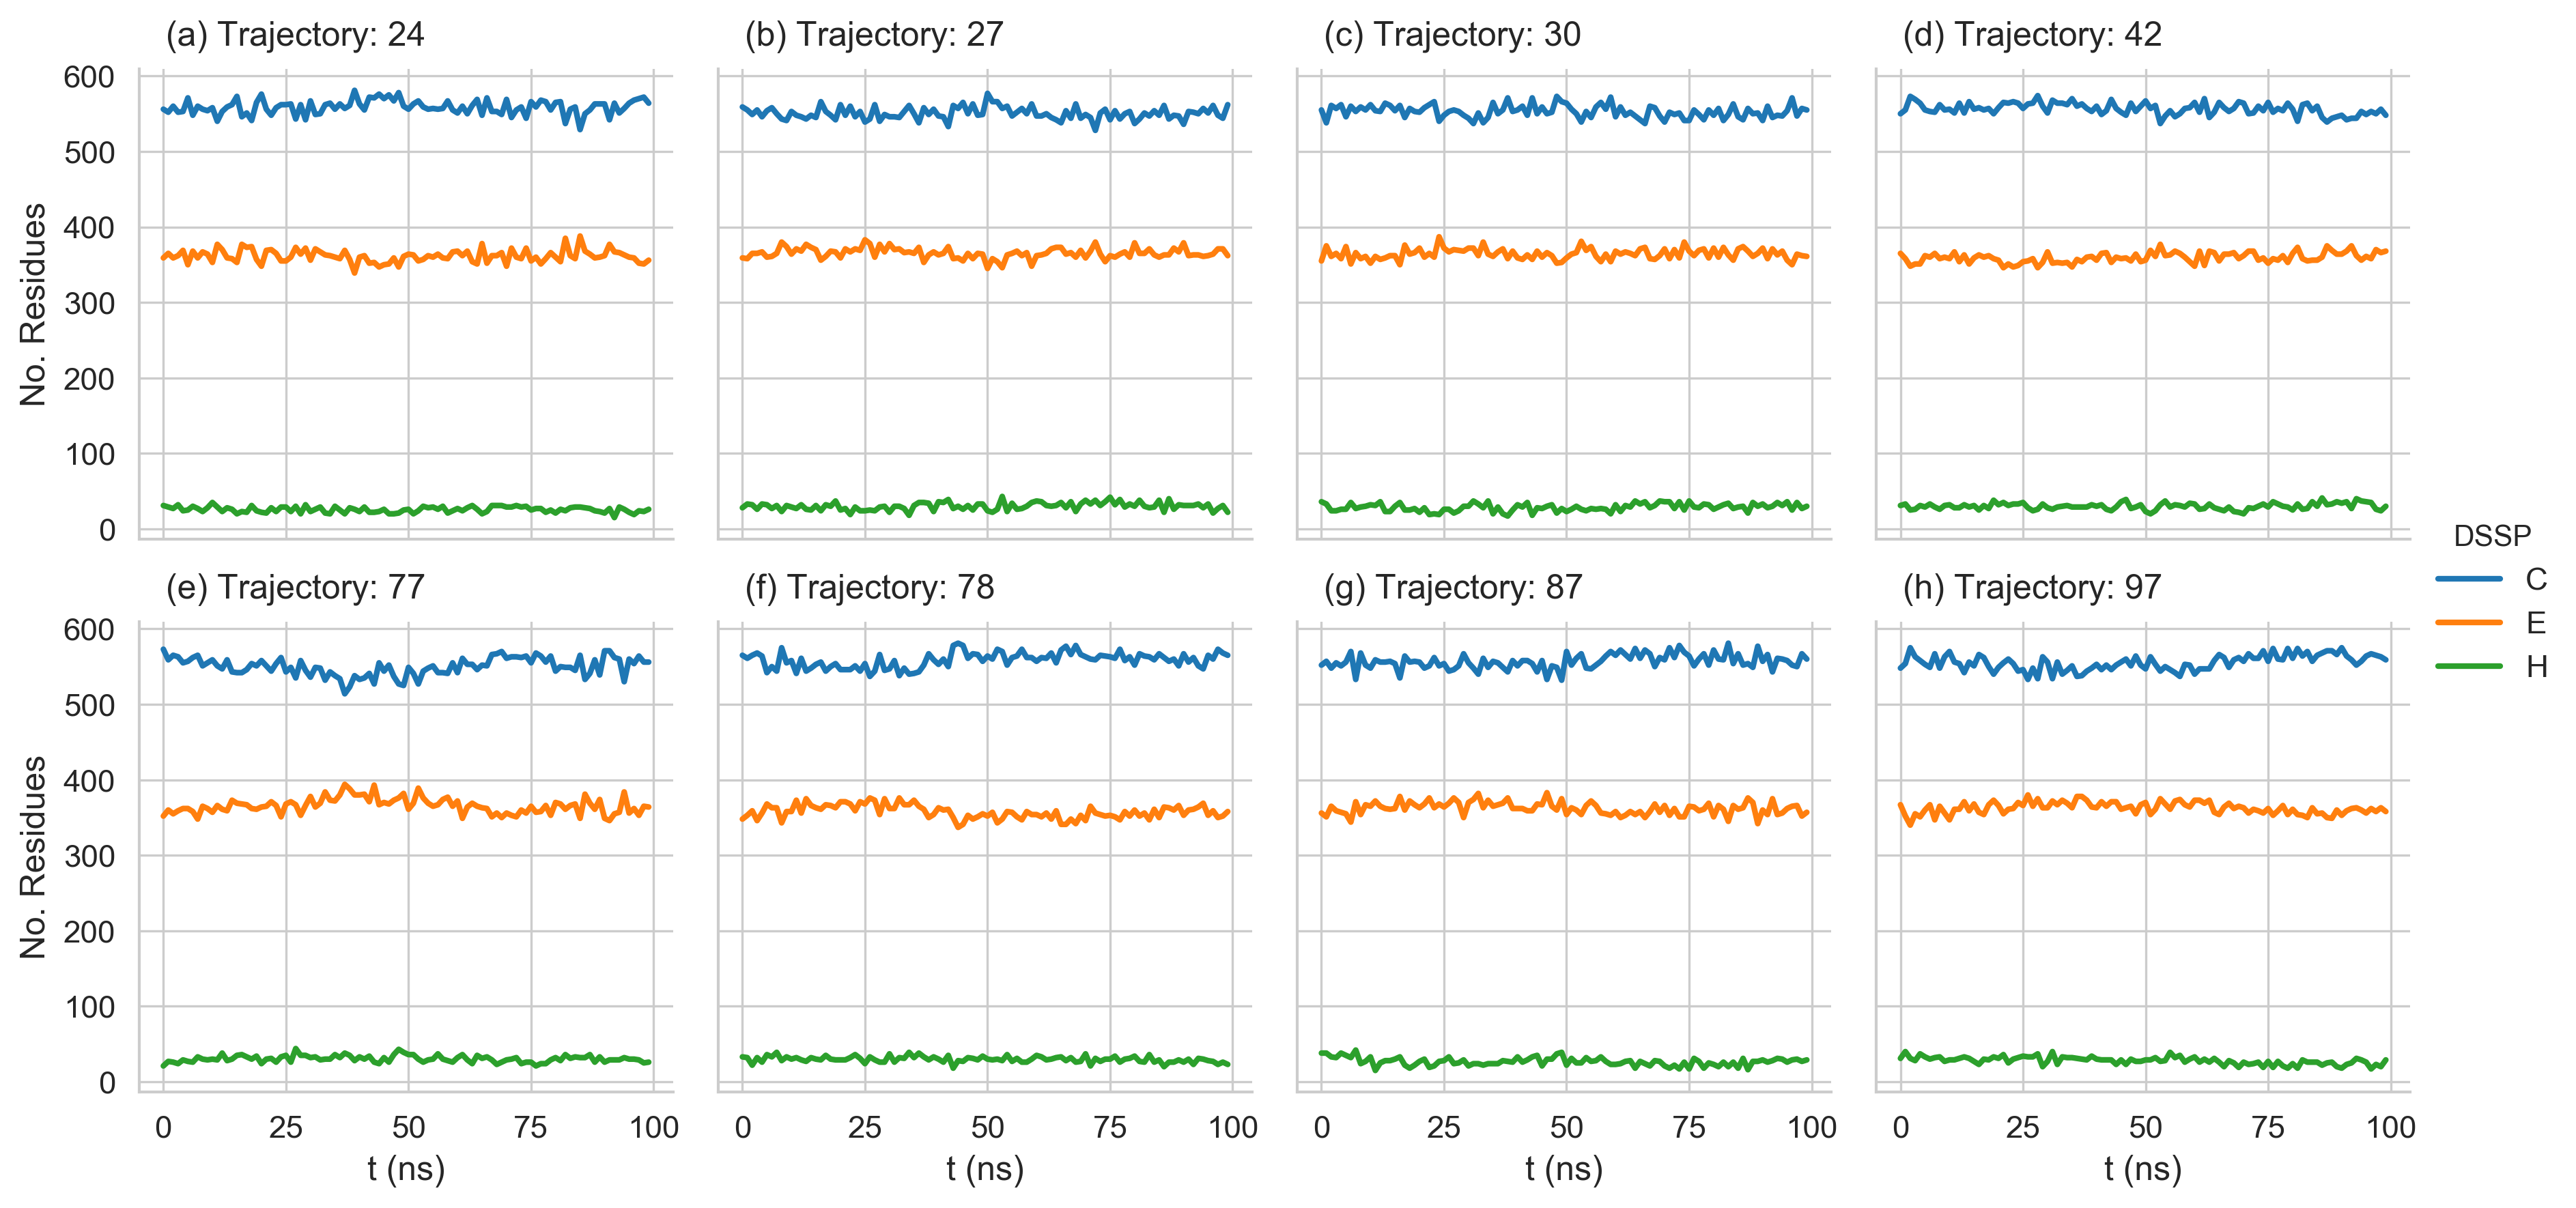
\includegraphics[width=0.9\textwidth]{chapters/aadh/figures/drift_trajs_dssp.png}
    \label{fig:dssp_trajs_sens}
\end{figure}

\begin{figure}
    \centering
    \mycaption{a;lkdjf;aklds}
    \label{fig:chain_d_loop}
    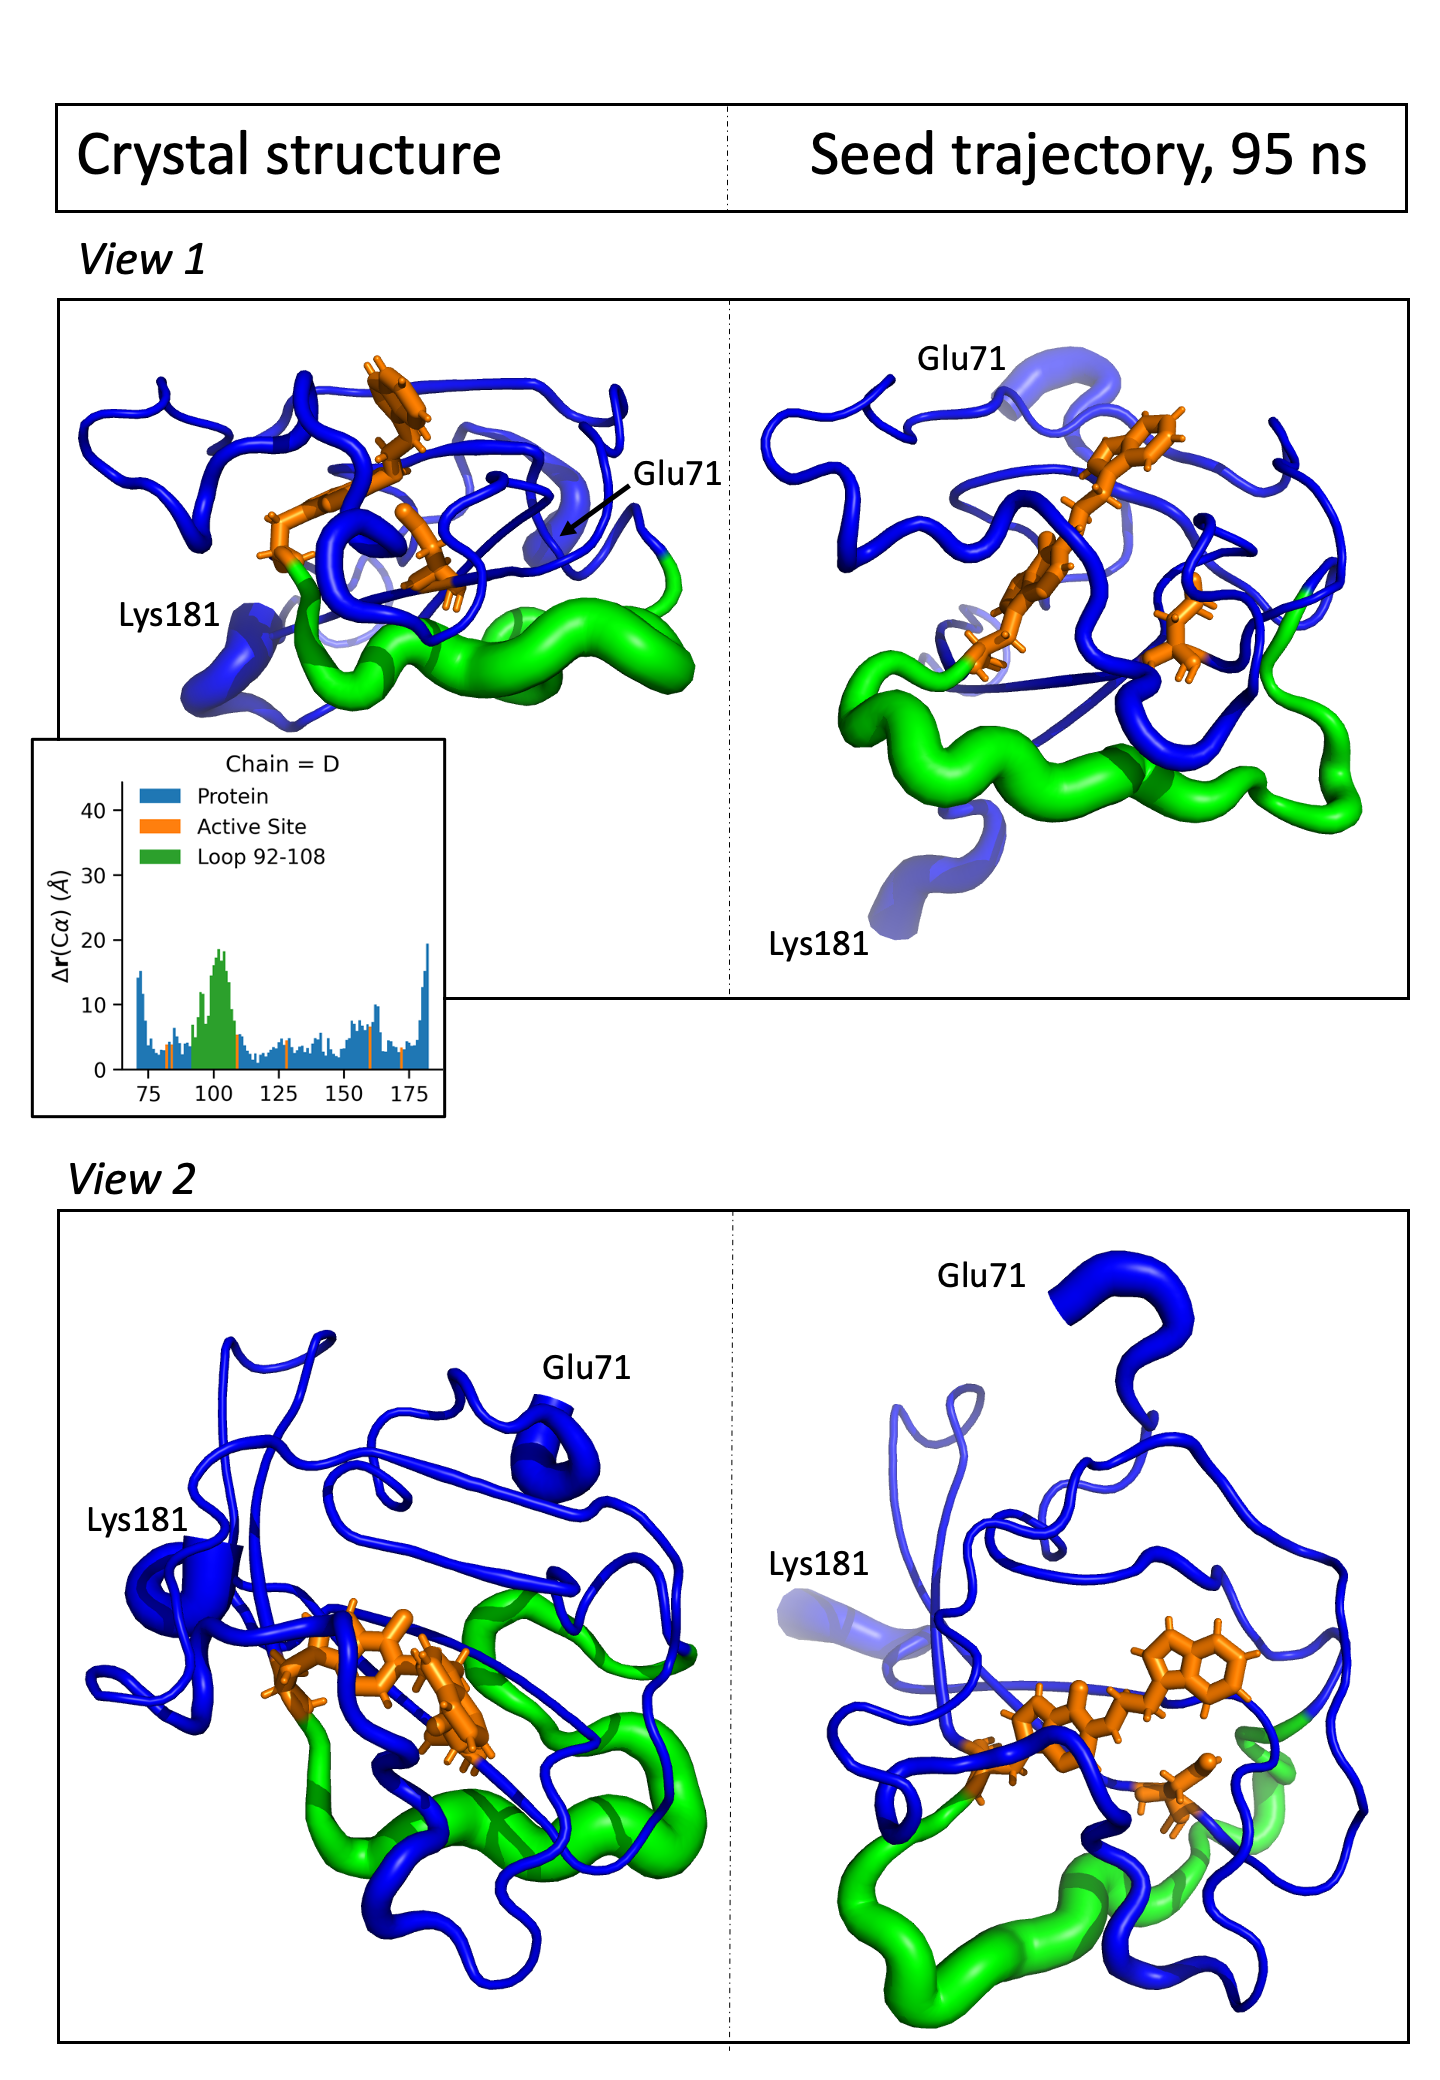
\includegraphics[height=0.9\textheight]{rmsd_seg_d.png}
\end{figure}

\section{MSM optimisation}

\subsection{Choosing $\tau$ and $k$}

\begin{figure}
    \centering
    \mycaption{The ratio of successive eigenvalues (panel (a)) and implied timescales (panel (b)) for a Markov state model with $\tau(\textrm{MSM})=\SI{2}{\nano\second}$, estimated using MCMC with $1000$ posterior samples. The TICA lag time was  $\tau=\SI{10}{\nano\second}$, with \SI{95}{\percent} of the variance/$m=8$ components retained. The number of cluster centres was $n=316$. The blue dots and error bars are the mean and \SI{95}{\percent} credible intervals.}
    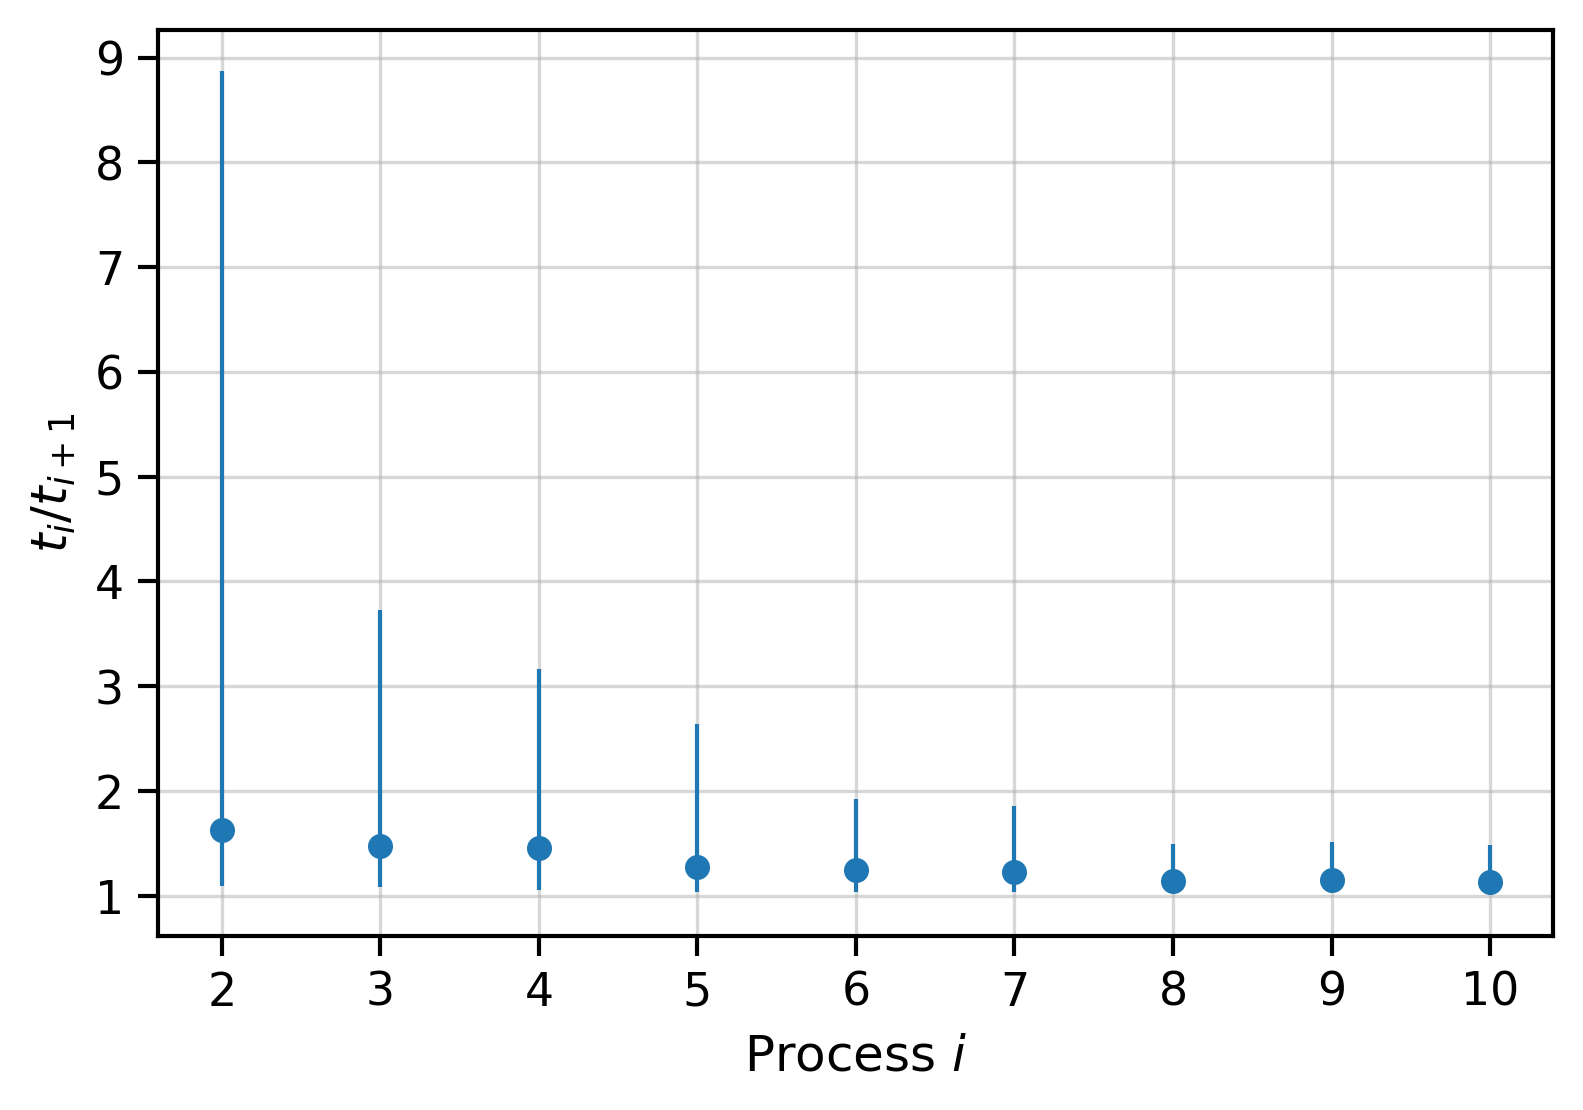
\includegraphics[width=0.8\textwidth]{chapters/aadh/figures/timescale_ratios_D_sens.png}
    \label{fig:ts_ratios_d_sens}
\end{figure}

\begin{figure}
    \centering
    \mycaption{The implied timescales and relative VAMP-2 scores as a function of the Markov lag time $\tau(\mathrm{MSM})$. The TICA lag time was set to $\tau=\SI{10}{\nano\second}$, with \SI{95}{\percent} of the variance retained meaning $m=8$ components were retained. The number of cluster centres was set to $n=316$. Panel (a) shows the first five implied timescales for $\SI{0}{\nano\second} < \tau(\mathrm{MSM}) < \SI{5}{\nano\second}$, panel (b) shows the first five implied timescales for $\SI{0}{\nano\second} < \tau(\mathrm{MSM}) < \SI{50}{\nano\second}$. The solid lines and coloured shaded areas are the mean and \SI{95}{\percent} credible intervals respectively, estimated using MCMC with $500$ posterior samples. The grey shaded area is the region for which the implied timescales are smaller than the lag time. Panel (c) and (d) show the VAMP-2 scores, scored on the first $2-5$ eigenvalues for the same ranges. The VAMP-2 scores are indexed to $1$ at their initial value. The colour coding is consistent between the implied timescale plots and VAMP-2 plots. So that $k=2$, in blue, is the score including the first eigenvalue $\lambda = 1$ and the eigenvalue of the longest implied timescale also shown in blue in panels (a) and (b). }
    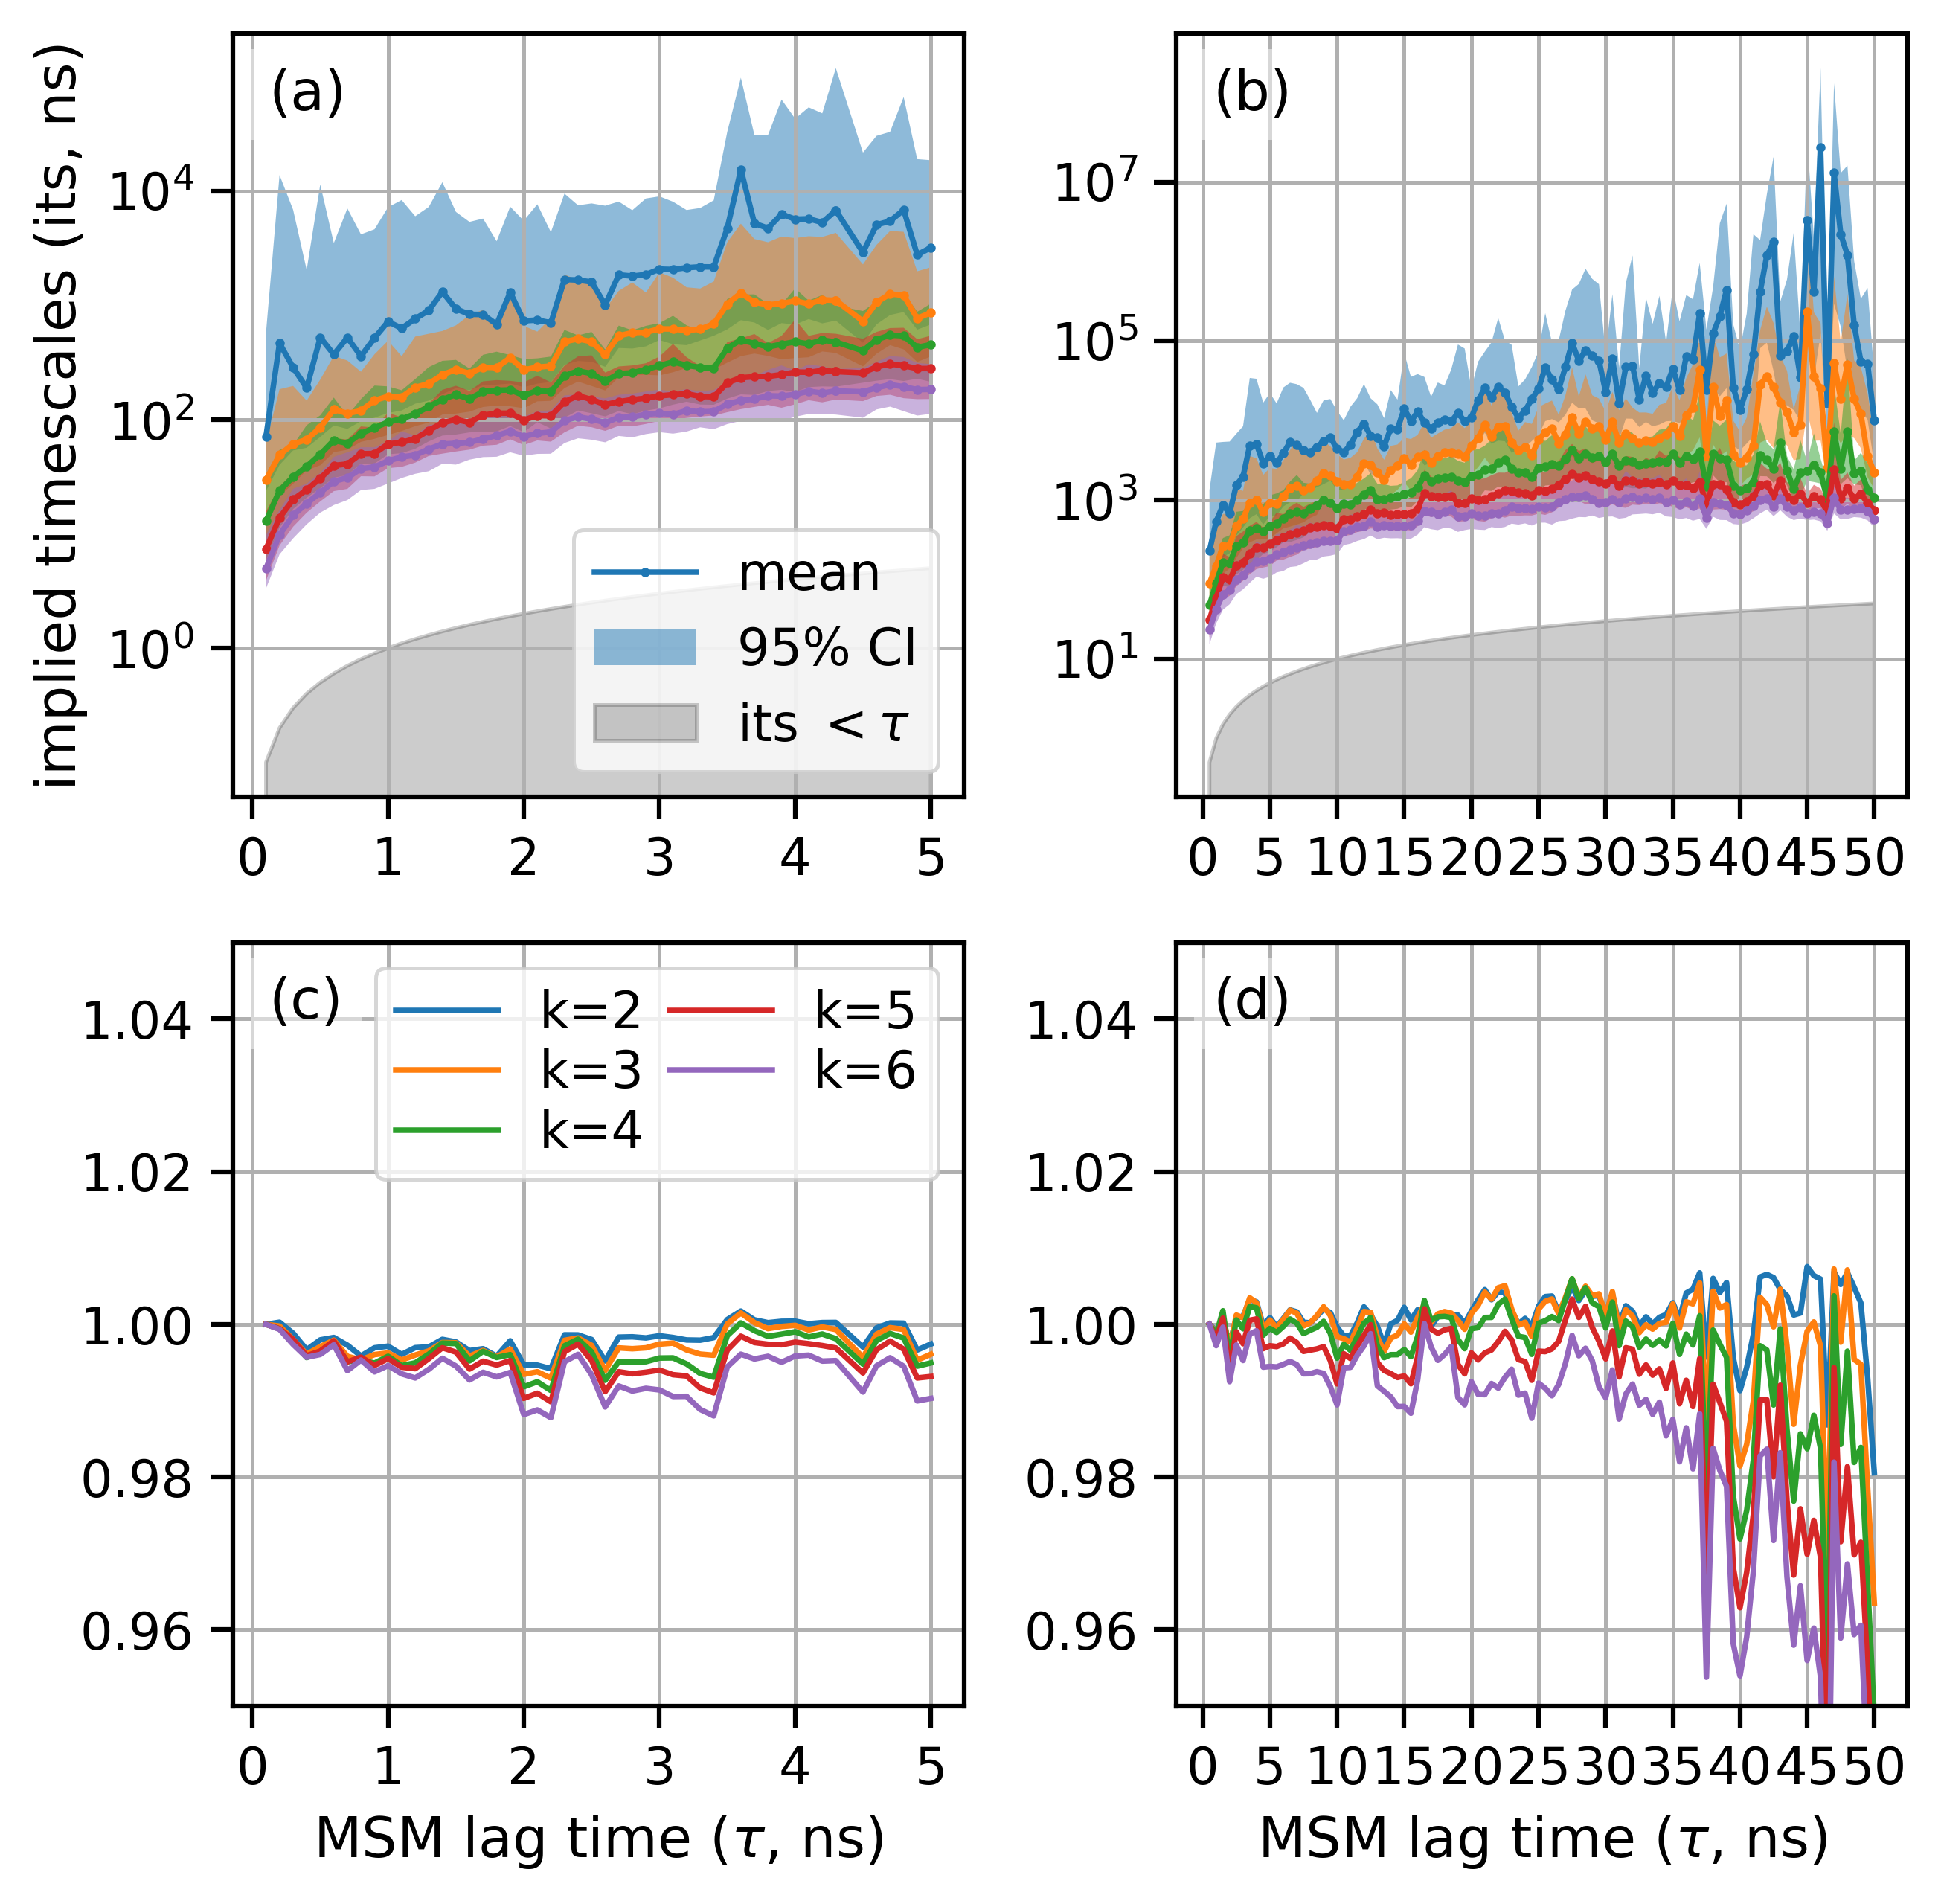
\includegraphics[width=0.8\textwidth]{chapters/aadh/figures/implied_timescales_D_sens.png}
    \label{fig:its_d_sens}
\end{figure}

\subsection{Response surface}\label{app:msm_rsm}

feature description. 


\section{Coarse graining models}

\subsection{Hidden state selection}
\begin{table}[]
    \centering
    \caption{Hidden state selection for AADH}
    \begin{tabular}{lrrrrrr}
    \toprule
              Case &  $g$ &   $d$ & $N_{\mathrm{obs}}$ &  $g^{\mathrm{rev}}$ &   Entropy &       ICL \\
    \midrule
         Base case &    2 &   620 &             98,000 &                   1 & 2.007e+00 & 1.070e+06 \\
         Base case &    3 &   932 &             98,000 &                   2 & 5.263e+00 & 1.009e+06 \\
         Base case &    4 & 1,245 &             98,000 &                   3 & 8.914e+02 & 9.375e+05 \\
         Base case &    5 & 1,559 &             98,000 &                   3 & 2.994e+02 & 9.036e+05 \\
         Base case &    6 & 1,874 &             98,000 &                   4 & 9.797e+02 & 8.715e+05 \\
         Base case &    7 & 2,190 &             98,000 &                   5 & 2.093e+03 & 8.491e+05 \\
         Base case &    8 & 2,507 &             98,000 &                   6 & 2.968e+03 & 8.342e+05 \\
         Base case &    9 & 2,825 &             98,000 &                   7 & 3.399e+03 & 8.312e+05 \\
         Base case &   10 & 3,144 &             98,000 &                   8 & 3.369e+03 & 8.083e+05 \\
         Base case &   11 & 3,464 &             98,000 &                   9 & 4.200e+03 & 7.966e+05 \\
         Base case &   12 & 3,785 &             98,000 &                  10 & 5.026e+03 & 7.847e+05 \\
         Base case &   13 & 4,107 &             98,000 &                  11 & 4.075e+03 & 7.936e+05 \\
         Base case &   14 & 4,430 &             98,000 &                  12 & 5.022e+03 & 7.891e+05 \\
         Base case &   15 & 4,754 &             98,000 &                  13 & 5.070e+03 & 7.854e+05 \\
         Base case &   16 & 5,079 &             98,000 &                  13 & 5.032e+03 & 7.870e+05 \\
         Base case &   17 & 5,405 &             98,000 &                  14 & 5.963e+03 & 7.801e+05 \\
         Base case &   18 & 5,732 &             98,000 &                  15 & 6.674e+03 & 7.785e+05 \\
         Base case &   19 & 6,060 &             98,000 &                  16 & 6.400e+03 & 7.786e+05 \\
         Base case &   20 & 6,389 &             98,000 &                  17 & 9.177e+03 & 7.806e+05 \\
     Sensitivity 1 &    2 &   608 &             80,000 &                   1 & 2.036e+02 & 1.040e+06 \\
     Sensitivity 1 &    5 & 1,529 &             80,000 &                   1 & 2.457e+03 & 9.361e+05 \\
     Sensitivity 1 &    6 & 1,838 &             80,000 &                   4 & 8.101e+03 & 9.287e+05 \\
     Sensitivity 1 &    8 & 2,459 &             80,000 &                   2 & 9.329e+03 & 9.233e+05 \\
     Sensitivity 2 &    2 &   220 &             98,000 &                   1 & 2.531e-02 & 8.224e+05 \\
     Sensitivity 2 &    3 &   332 &             98,000 &                   2 & 7.167e+02 & 7.139e+05 \\
     Sensitivity 2 &    4 &   445 &             98,000 &                   3 & 1.679e+02 & 6.509e+05 \\
     Sensitivity 2 &    5 &   559 &             98,000 &                   4 & 1.086e+03 & 6.165e+05 \\
     Sensitivity 2 &    6 &   674 &             98,000 &                   5 & 1.409e+03 & 5.951e+05 \\
     Sensitivity 2 &    7 &   790 &             98,000 &                   5 & 1.612e+03 & 5.874e+05 \\
     Sensitivity 2 &    8 &   907 &             98,000 &                   6 & 1.672e+03 & 5.776e+05 \\
     Sensitivity 2 &    9 & 1,025 &             98,000 &                   6 & 1.594e+03 & 5.718e+05 \\
     Sensitivity 2 &   10 & 1,144 &             98,000 &                   7 & 1.873e+03 & 5.676e+05 \\
     Sensitivity 2 &   11 & 1,264 &             98,000 &                   8 & 2.759e+03 & 5.637e+05 \\
     Sensitivity 2 &   12 & 1,385 &             98,000 &                   8 & 2.278e+03 & 5.600e+05 \\
     Sensitivity 2 &   13 & 1,507 &             98,000 &                   8 & 2.382e+03 & 5.552e+05 \\
     Sensitivity 2 &   14 & 1,630 &             98,000 &                   9 & 2.861e+03 & 5.493e+05 \\
     Sensitivity 2 &   15 & 1,754 &             98,000 &                  10 & 3.087e+03 & 5.483e+05 \\
     Sensitivity 2 &   16 & 1,879 &             98,000 &                  11 & 3.710e+03 & 5.451e+05 \\
     Sensitivity 2 &   17 & 2,005 &             98,000 &                  11 & 8.145e+03 & 5.369e+05 \\
     Sensitivity 2 &   18 & 2,132 &             98,000 &                  11 & 8.196e+03 & 5.361e+05 \\
     Sensitivity 2 &   19 & 2,260 &             98,000 &                  13 & 8.662e+03 & 5.294e+05 \\
     Sensitivity 2 &   20 & 2,389 &             98,000 &                  12 & 8.653e+03 & 5.299e+05 \\
     Sensitivity 3 &    2 &   620 &             98,000 &                   2 & 8.322e+01 & 9.751e+05 \\
     Sensitivity 3 &    3 &   932 &             98,000 &                   3 & 1.249e+02 & 9.290e+05 \\
     Sensitivity 3 &    4 & 1,245 &             98,000 &                   4 & 1.479e+03 & 9.097e+05 \\
     Sensitivity 3 &    5 & 1,559 &             98,000 &                   5 & 4.028e+03 & 8.949e+05 \\
     Sensitivity 3 &    6 & 1,874 &             98,000 &                   6 & 3.845e+03 & 8.834e+05 \\
     Sensitivity 3 &    7 & 2,190 &             98,000 &                   7 & 3.899e+03 & 8.806e+05 \\
     Sensitivity 3 &    8 & 2,507 &             98,000 &                   7 & 5.300e+03 & 8.774e+05 \\
     Sensitivity 3 &    9 & 2,825 &             98,000 &                   6 & 4.499e+03 & 8.720e+05 \\
     Sensitivity 3 &   10 & 3,144 &             98,000 &                   6 & 4.837e+03 & 8.734e+05 \\
     Sensitivity 3 &   11 & 3,464 &             98,000 &                   8 & 1.090e+04 & 8.636e+05 \\
     Sensitivity 3 &   12 & 3,785 &             98,000 &                  10 & 9.241e+03 & 8.664e+05 \\
     Sensitivity 3 &   13 & 4,107 &             98,000 &                  12 & 9.855e+03 & 8.619e+05 \\
     Sensitivity 3 &   14 & 4,430 &             98,000 &                  12 & 9.923e+03 & 8.622e+05 \\
     Sensitivity 3 &   15 & 4,754 &             98,000 &                  13 & 1.040e+04 & 8.613e+05 \\
     Sensitivity 3 &   16 & 5,079 &             98,000 &                  14 & 1.201e+04 & 8.613e+05 \\
     Sensitivity 3 &   17 & 5,405 &             98,000 &                  15 & 1.240e+04 & 8.641e+05 \\
     Sensitivity 3 &   18 & 5,732 &             98,000 &                  16 & 1.285e+04 & 8.612e+05 \\
     Sensitivity 3 &   19 & 6,060 &             98,000 &                  17 & 1.385e+04 & 8.621e+05 \\
     Sensitivity 3 &   20 & 6,389 &             98,000 &                  18 & 1.401e+04 & 8.655e+05 \\
    \bottomrule
    \end{tabular}
    \label{tab:aadh_h_state_selection}
\end{table}

\subsection{Base Case Model}
\begin{table}
    \centering
    \caption{Gelman-Rubin statistics for the hidden state transition matrix elements for the `base case' Bayesian HMM of AADH. The model was estimated with four independent MCMC chains with $4000$ posterior samples, taken after neglecting the first $1000$ samples. }
    \label{tab:aadh_base_case_rhat}
    \begin{tabular}{|r|r|r||r|r|r|}
    \hline
    $i$ & $j$ & $\hat{R}$ & $i$ & $j$ & $\hat{R}$ \\
    \hline\hline
      1 &   1 &      1.02 &   8 &  11 &      1.01 \\
      1 &   4 &      1.00 &   8 &  12 &      1.06 \\
      1 &   9 &      1.00 &   8 &  13 &      1.04 \\
      1 &  10 &      1.01 &   9 &   1 &      1.00 \\
      1 &  13 &      1.00 &   9 &   4 &      1.10 \\
      1 &  14 &      1.00 &   9 &   5 &      1.00 \\
      1 &  15 &      1.03 &   9 &   7 &      1.07 \\
      2 &   2 &      1.03 &   9 &   8 &      1.00 \\
      2 &   3 &      1.05 &   9 &   9 &      1.10 \\
      2 &   5 &      1.04 &   9 &  10 &      1.00 \\
      2 &   6 &      1.00 &   9 &  12 &      1.00 \\
      2 &   7 &      1.00 &   9 &  13 &      1.00 \\
      2 &   8 &      1.00 &  10 &   1 &      1.01 \\
      2 &  12 &      1.00 &  10 &   4 &      1.00 \\
      2 &  13 &      1.00 &  10 &   8 &      1.01 \\
      3 &   2 &      1.05 &  10 &   9 &      1.00 \\
      3 &   3 &      1.00 &  10 &  10 &      1.04 \\
      3 &   5 &      1.01 &  10 &  12 &      1.01 \\
      3 &   6 &      1.00 &  10 &  13 &      1.00 \\
      4 &   1 &      1.00 &  10 &  14 &      1.02 \\
      4 &   4 &      1.02 &  10 &  15 &      1.06 \\
      4 &   5 &      1.04 &  11 &   7 &      1.00 \\
      4 &   7 &      1.00 &  11 &   8 &      1.01 \\
      4 &   8 &      1.00 &  11 &  11 &      1.00 \\
      4 &   9 &      1.02 &  11 &  12 &      1.02 \\
      4 &  10 &      1.02 &  11 &  13 &      1.00 \\
      4 &  12 &      1.00 &  12 &   2 &      1.00 \\
      4 &  13 &      1.00 &  12 &   4 &      1.00 \\
      4 &  14 &      1.00 &  12 &   5 &      1.00 \\
      4 &  15 &      1.00 &  12 &   7 &      1.00 \\
      5 &   2 &      1.01 &  12 &   8 &      1.04 \\
      5 &   3 &      1.01 &  12 &   9 &      1.00 \\
      5 &   4 &      1.05 &  12 &  10 &      1.01 \\
      5 &   5 &      1.00 &  12 &  11 &      1.02 \\
      5 &   6 &      1.01 &  12 &  12 &      1.03 \\
      5 &   7 &      1.00 &  12 &  13 &      1.02 \\
      5 &   8 &      1.00 &  13 &   1 &      1.00 \\
      5 &   9 &      1.01 &  13 &   2 &      1.00 \\
      5 &  12 &      1.00 &  13 &   4 &      1.00 \\
      5 &  13 &      1.00 &  13 &   5 &      1.00 \\
      6 &   2 &      1.00 &  13 &   7 &      1.01 \\
      6 &   3 &      1.00 &  13 &   8 &      1.03 \\
      6 &   5 &      1.03 &  13 &   9 &      1.00 \\
      6 &   6 &      1.03 &  13 &  10 &      1.00 \\
      7 &   2 &      1.00 &  13 &  11 &      1.00 \\
      7 &   4 &      1.00 &  13 &  12 &      1.02 \\
      7 &   5 &      1.00 &  13 &  13 &      1.02 \\
      7 &   7 &      1.03 &  13 &  15 &      1.00 \\
      7 &   8 &      1.02 &  14 &   1 &      1.00 \\
      7 &   9 &      1.06 &  14 &   4 &      1.00 \\
      7 &  11 &      1.00 &  14 &  10 &      1.02 \\
      7 &  12 &      1.00 &  14 &  14 &      1.02 \\
      7 &  13 &      1.01 &  14 &  15 &      1.02 \\
      8 &   2 &      1.00 &  15 &   1 &      1.04 \\
      8 &   4 &      1.00 &  15 &   4 &      1.00 \\
      8 &   5 &      1.00 &  15 &  10 &      1.09 \\
      8 &   7 &      1.03 &  15 &  13 &      1.00 \\
      8 &   8 &      1.08 &  15 &  14 &      1.04 \\
      8 &   9 &      1.00 &  15 &  15 &      1.07 \\
      8 &  10 &      1.01 &   - &   - &         - \\
    \hline
    \end{tabular}
\end{table}

\begin{table}
    \centering
    \mycaption{Rate Matrix}
    \label{tab:base_case_rate_matrix}
    \begin{tabular}{|rrl||rrl||rrl|}
    \hline
     $i$ &  $j$ &          $k_{ij}$ &  $i$ &  $j$ &           $k_{ij}$ &  $i$ &  $j$ &            $k_{ij}$ \\
    \hline\hline
       1 &    2 &    0.3 (0.0, 1.3) &    3 &   12 &     0.1 (0.0, 0.2) &    7 &    9 &      0.0 (0.0, 0.0) \\
       2 &    1 &    0.0 (0.0, 0.2) &   12 &    3 &     0.0 (0.0, 0.1) &    9 &    7 &      0.0 (0.0, 0.0) \\
       1 &    3 &  22.2 (0.5, 83.5) &    3 &   13 &    3.1 (0.1, 12.6) &    7 &   10 &      0.5 (0.1, 1.2) \\
       3 &    1 &   9.1 (0.8, 28.1) &   13 &    3 &     0.8 (0.0, 4.2) &   10 &    7 &      0.4 (0.1, 1.2) \\
       1 &    4 &    0.0 (0.0, 0.0) &    3 &   14 &     0.1 (0.0, 0.4) &    7 &   11 &    10.5 (5.3, 17.8) \\
       4 &    1 &    0.0 (0.0, 0.0) &   14 &    3 &     0.0 (0.0, 0.1) &   11 &    7 &     5.6 (2.0, 11.5) \\
       1 &    5 &    0.0 (0.0, 0.0) &    3 &   15 &    0.0 (-0.0, 0.0) &    7 &   12 &      0.1 (0.0, 0.2) \\
       5 &    1 &    0.0 (0.0, 0.0) &   15 &    3 &    0.0 (-0.0, 0.0) &   12 &    7 &      0.1 (0.0, 0.2) \\
       1 &    6 &    0.0 (0.0, 0.0) &    4 &    5 &  17.1 (10.7, 25.6) &    7 &   13 &     0.4 (-0.2, 2.9) \\
       6 &    1 &    0.0 (0.0, 0.0) &    5 &    4 &   12.1 (6.5, 19.8) &   13 &    7 &     0.3 (-0.2, 2.2) \\
       1 &    7 &    0.0 (0.0, 0.0) &    4 &    6 &     0.1 (0.0, 0.2) &    7 &   14 &     0.4 (-0.2, 2.4) \\
       7 &    1 &    0.0 (0.0, 0.0) &    6 &    4 &     0.3 (0.0, 0.9) &   14 &    7 &     0.3 (-0.2, 2.0) \\
       1 &    8 &   0.0 (-0.0, 0.1) &    4 &    7 &    0.0 (-0.3, 1.0) &    7 &   15 &     0.0 (-0.0, 0.0) \\
       8 &    1 &    0.0 (0.0, 0.0) &    7 &    4 &    0.0 (-0.3, 1.0) &   15 &    7 &     0.0 (-0.0, 0.0) \\
       1 &    9 &  2.6 (-2.1, 22.8) &    4 &    8 &     0.0 (0.0, 0.0) &    8 &    9 &     0.0 (-0.0, 0.1) \\
       9 &    1 &  1.5 (-1.0, 12.5) &    8 &    4 &     0.0 (0.0, 0.0) &    9 &    8 &     0.0 (-0.0, 0.1) \\
       1 &   10 &    0.1 (0.0, 0.7) &    4 &    9 &     0.0 (0.0, 0.0) &    8 &   10 &  61.1 (22.5, 112.7) \\
      10 &    1 &    0.0 (0.0, 0.1) &    9 &    4 &     0.0 (0.0, 0.0) &   10 &    8 &    35.6 (8.3, 78.2) \\
       1 &   11 &    0.0 (0.0, 0.0) &    4 &   10 &     0.0 (0.0, 0.0) &    8 &   11 &      0.2 (0.0, 0.5) \\
      11 &    1 &    0.0 (0.0, 0.0) &   10 &    4 &     0.0 (0.0, 0.0) &   11 &    8 &      0.1 (0.0, 0.2) \\
       1 &   12 &    0.0 (0.0, 0.0) &    4 &   11 &     0.0 (0.0, 0.0) &    8 &   12 &     0.5 (-1.0, 1.7) \\
      12 &    1 &    0.0 (0.0, 0.0) &   11 &    4 &     0.0 (0.0, 0.0) &   12 &    8 &     0.2 (-0.4, 0.8) \\
       1 &   13 &    0.1 (0.0, 0.4) &    4 &   12 &     0.0 (0.0, 0.0) &    8 &   13 &     0.0 (-0.0, 0.0) \\
      13 &    1 &    0.0 (0.0, 0.0) &   12 &    4 &     0.0 (0.0, 0.0) &   13 &    8 &     0.0 (-0.0, 0.0) \\
       1 &   14 &    0.0 (0.0, 0.0) &    4 &   13 &     0.0 (0.0, 0.0) &    8 &   14 &      0.0 (0.0, 0.0) \\
      14 &    1 &    0.0 (0.0, 0.0) &   13 &    4 &     0.0 (0.0, 0.0) &   14 &    8 &      0.0 (0.0, 0.0) \\
       1 &   15 &    0.0 (0.0, 0.0) &    4 &   14 &     0.0 (0.0, 0.0) &    8 &   15 &      0.0 (0.0, 0.0) \\
      15 &    1 &    0.0 (0.0, 0.0) &   14 &    4 &     0.0 (0.0, 0.0) &   15 &    8 &      0.0 (0.0, 0.0) \\
       2 &    3 &   5.4 (0.2, 16.8) &    4 &   15 &     0.0 (0.0, 0.0) &    9 &   10 &      0.2 (0.0, 0.8) \\
       3 &    2 &  12.0 (1.6, 32.2) &   15 &    4 &     0.0 (0.0, 0.0) &   10 &    9 &      0.0 (0.0, 0.2) \\
       2 &    4 &    0.0 (0.0, 0.0) &    5 &    6 &    5.3 (1.5, 11.4) &    9 &   11 &      0.0 (0.0, 0.0) \\
       4 &    2 &    0.0 (0.0, 0.0) &    6 &    5 &   25.8 (4.5, 63.3) &   11 &    9 &      0.0 (0.0, 0.0) \\
       2 &    5 &    0.0 (0.0, 0.0) &    5 &    7 &   10.9 (5.7, 18.2) &    9 &   12 &      0.0 (0.0, 0.0) \\
       5 &    2 &    0.0 (0.0, 0.0) &    7 &    5 &   15.0 (6.8, 27.1) &   12 &    9 &      0.0 (0.0, 0.0) \\
       2 &    6 &    0.0 (0.0, 0.0) &    5 &    8 &     0.1 (0.0, 0.2) &    9 &   13 &      0.1 (0.0, 0.5) \\
       6 &    2 &    0.0 (0.0, 0.0) &    8 &    5 &     0.2 (0.0, 0.5) &   13 &    9 &      0.0 (0.0, 0.1) \\
       2 &    7 &    0.0 (0.0, 0.0) &    5 &    9 &     0.0 (0.0, 0.0) &    9 &   14 &      0.0 (0.0, 0.0) \\
       7 &    2 &    0.0 (0.0, 0.0) &    9 &    5 &     0.0 (0.0, 0.0) &   14 &    9 &      0.0 (0.0, 0.0) \\
       2 &    8 &    0.0 (0.0, 0.0) &    5 &   10 &     0.0 (0.0, 0.0) &    9 &   15 &      0.0 (0.0, 0.0) \\
       8 &    2 &    0.0 (0.0, 0.0) &   10 &    5 &     0.0 (0.0, 0.0) &   15 &    9 &      0.0 (0.0, 0.0) \\
       2 &    9 &    0.1 (0.0, 0.5) &    5 &   11 &     0.1 (0.1, 0.3) &   10 &   11 &     1.0 (-0.1, 4.5) \\
       9 &    2 &    0.4 (0.0, 1.3) &   11 &    5 &     0.1 (0.0, 0.2) &   11 &   10 &     0.7 (-0.1, 2.9) \\
       2 &   10 &    0.0 (0.0, 0.2) &    5 &   12 &     0.0 (0.0, 0.0) &   10 &   12 &    10.2 (2.8, 22.5) \\
      10 &    2 &    0.0 (0.0, 0.1) &   12 &    5 &     0.0 (0.0, 0.0) &   12 &   10 &     7.1 (1.8, 16.7) \\
       2 &   11 &    0.0 (0.0, 0.0) &    5 &   13 &    0.0 (-0.0, 0.0) &   10 &   13 &     0.0 (-0.0, 0.0) \\
      11 &    2 &    0.0 (0.0, 0.0) &   13 &    5 &    0.0 (-0.0, 0.0) &   13 &   10 &     0.0 (-0.0, 0.0) \\
       2 &   12 &    0.0 (0.0, 0.0) &    5 &   14 &    0.0 (-0.0, 0.0) &   10 &   14 &      0.1 (0.0, 0.2) \\
      12 &    2 &    0.0 (0.0, 0.0) &   14 &    5 &    0.0 (-0.0, 0.0) &   14 &   10 &      0.0 (0.0, 0.2) \\
       2 &   13 &    0.0 (0.0, 0.1) &    5 &   15 &     0.0 (0.0, 0.0) &   10 &   15 &      0.0 (0.0, 0.0) \\
      13 &    2 &    0.0 (0.0, 0.1) &   15 &    5 &     0.0 (0.0, 0.0) &   15 &   10 &      0.0 (0.0, 0.0) \\
       2 &   14 &    0.0 (0.0, 0.0) &    6 &    7 &    7.2 (0.1, 23.1) &   11 &   12 &    10.8 (4.8, 19.5) \\
      14 &    2 &    0.0 (0.0, 0.0) &    7 &    6 &     2.0 (0.0, 6.2) &   12 &   11 &    11.1 (3.5, 23.6) \\
       2 &   15 &    0.0 (0.0, 0.0) &    6 &    8 &    0.1 (-0.0, 0.2) &   11 &   13 &     8.2 (3.0, 16.1) \\
      15 &    2 &    0.0 (0.0, 0.0) &    8 &    6 &    0.0 (-0.0, 0.1) &   13 &   11 &     9.4 (2.3, 21.5) \\
       3 &    4 &    0.0 (0.0, 0.0) &    6 &    9 &     0.0 (0.0, 0.0) &   11 &   14 &     7.4 (1.9, 16.4) \\
       4 &    3 &    0.0 (0.0, 0.0) &    9 &    6 &     0.0 (0.0, 0.0) &   14 &   11 &    10.5 (2.1, 25.6) \\
       3 &    5 &    0.0 (0.0, 0.0) &    6 &   10 &    0.0 (-0.0, 0.0) &   11 &   15 &      0.1 (0.0, 0.2) \\
       5 &    3 &    0.0 (0.0, 0.0) &   10 &    6 &     0.0 (0.0, 0.0) &   15 &   11 &      0.1 (0.0, 0.2) \\
       3 &    6 &    0.0 (0.0, 0.0) &    6 &   11 &   2.5 (-0.1, 10.9) &   12 &   13 &      0.2 (0.1, 0.6) \\
       6 &    3 &    0.0 (0.0, 0.0) &   11 &    6 &    0.4 (-0.0, 1.9) &   13 &   12 &      0.2 (0.1, 0.7) \\
       3 &    7 &   0.0 (-0.0, 0.1) &    6 &   12 &    0.0 (-0.0, 0.1) &   12 &   14 &     4.3 (0.4, 12.9) \\
       7 &    3 &    0.0 (0.0, 0.0) &   12 &    6 &    0.0 (-0.0, 0.0) &   14 &   12 &     5.8 (0.6, 16.2) \\
       3 &    8 &   0.2 (-0.9, 4.4) &    6 &   13 &    0.0 (-0.0, 0.1) &   12 &   15 &      0.0 (0.0, 0.1) \\
       8 &    3 &   0.1 (-0.6, 2.4) &   13 &    6 &    0.0 (-0.0, 0.0) &   15 &   12 &      0.0 (0.0, 0.1) \\
       3 &    9 &  21.8 (6.3, 48.2) &    6 &   14 &    0.0 (-0.0, 0.1) &   13 &   14 &    24.8 (7.0, 54.6) \\
       9 &    3 &  31.5 (6.5, 72.6) &   14 &    6 &    0.0 (-0.0, 0.0) &   14 &   13 &   30.3 (10.6, 64.7) \\
       3 &   10 &   5.9 (0.3, 19.7) &    6 &   15 &     0.0 (0.0, 0.0) &   13 &   15 &     2.3 (-0.4, 9.4) \\
      10 &    3 &    2.0 (0.0, 8.5) &   15 &    6 &     0.0 (0.0, 0.0) &   15 &   13 &     1.5 (-0.3, 8.6) \\
       3 &   11 &    0.0 (0.0, 0.1) &    7 &    8 &    7.9 (3.3, 14.4) &   14 &   15 &     6.4 (0.9, 15.5) \\
      11 &    3 &    0.0 (0.0, 0.0) &    8 &    7 &   11.6 (2.8, 27.8) &   15 &   14 &     3.8 (0.0, 15.4) \\
    \hline
    \end{tabular}
\end{table}

\begin{table}
    \centering
    \mycaption{Stationary distribution}
    \label{tab:my_label}
    \begin{tabular}{|rl|}
    \hline
     $i$ & $\tilde{\pi_{i}}$ \\
    \hline\hline
       1 &   3.2 (0.0, 44.3) \\
       2 &  10.3 (0.1, 73.4) \\
       3 &   2.5 (0.1, 12.9) \\
       4 &   4.5 (0.4, 13.3) \\
       5 &   6.3 (0.5, 16.7) \\
       6 &    1.6 (0.1, 5.8) \\
       7 &   4.5 (0.4, 10.6) \\
       8 &   3.5 (0.3, 10.3) \\
       9 &   2.3 (0.0, 14.8) \\
      10 &   6.4 (0.6, 18.2) \\
      11 &   8.4 (0.8, 17.8) \\
      12 &   9.0 (0.9, 22.8) \\
      13 &   7.9 (0.9, 19.9) \\
      14 &   6.3 (0.7, 15.3) \\
      15 &  23.4 (1.6, 91.3) \\
    \hline
    \end{tabular}
\end{table}

\subsection{Sensitivity 2}

\begin{table}
    \centering
    \mycaption{Sensitivity 2 Gelman Rubin}
    \begin{tabular}{|rrl||rrl||rrl|}
    \hline
     $i$ &  $j$ & $\hat{R}$ &  $i$ &  $j$ & $\hat{R}$ &  $i$ &  $j$ & $\hat{R}$ \\
    \hline\hline
       1 &    1 &      1.01 &    4 &   13 &      1.00 &    9 &    6 &      1.06 \\
       1 &    2 &      1.03 &    5 &    1 &      1.01 &    9 &    7 &      1.00 \\
       1 &    3 &      1.00 &    5 &    2 &      1.01 &    9 &    8 &      1.01 \\
       1 &    4 &      1.00 &    5 &    3 &      1.02 &    9 &    9 &      1.01 \\
       1 &    5 &      1.00 &    5 &    5 &      1.13 &    9 &   10 &      1.01 \\
       1 &    6 &      1.00 &    5 &   12 &      1.14 &    9 &   11 &      1.02 \\
       1 &    7 &      1.00 &    6 &    1 &      1.01 &    9 &   13 &      1.01 \\
       1 &    8 &      1.00 &    6 &    2 &      1.00 &   10 &    1 &      1.00 \\
       1 &    9 &      1.00 &    6 &    3 &      1.01 &   10 &    2 &      1.00 \\
       1 &   10 &      1.00 &    6 &    4 &      1.02 &   10 &    4 &      1.00 \\
       1 &   11 &      1.00 &    6 &    6 &      1.07 &   10 &    6 &      1.17 \\
       1 &   12 &      1.00 &    6 &    7 &      1.03 &   10 &    7 &      1.17 \\
       2 &    1 &      1.02 &    6 &    8 &      1.01 &   10 &    8 &      1.06 \\
       2 &    2 &      1.12 &    6 &    9 &      1.07 &   10 &    9 &      1.01 \\
       2 &    3 &      1.10 &    6 &   10 &      1.04 &   10 &   10 &      1.01 \\
       2 &    4 &      1.00 &    6 &   11 &      1.19 &   10 &   11 &      1.16 \\
       2 &    5 &      1.00 &    6 &   13 &      1.01 &   10 &   13 &      1.00 \\
       2 &    6 &      1.04 &    7 &    1 &      1.00 &   11 &    1 &      1.00 \\
       2 &    7 &      1.11 &    7 &    2 &      1.10 &   11 &    2 &      1.00 \\
       2 &    8 &      1.00 &    7 &    3 &      1.00 &   11 &    3 &      1.00 \\
       2 &    9 &      1.00 &    7 &    4 &      1.00 &   11 &    4 &      1.00 \\
       2 &   10 &      1.00 &    7 &    6 &      1.21 &   11 &    6 &      1.28 \\
       2 &   11 &      1.00 &    7 &    7 &      1.04 &   11 &    7 &      1.30 \\
       2 &   12 &      1.04 &    7 &    8 &      1.00 &   11 &    8 &      1.01 \\
       3 &    1 &      1.00 &    7 &    9 &      1.00 &   11 &    9 &      1.02 \\
       3 &    2 &      1.04 &    7 &   10 &      1.16 &   11 &   10 &      1.15 \\
       3 &    3 &      1.05 &    7 &   11 &      1.28 &   11 &   11 &      1.03 \\
       3 &    5 &      1.08 &    7 &   13 &      1.00 &   11 &   13 &      1.00 \\
       3 &    6 &      1.00 &    8 &    1 &      1.00 &   12 &    1 &      1.01 \\
       3 &    7 &      1.00 &    8 &    2 &      1.00 &   12 &    2 &      1.08 \\
       3 &   11 &      1.00 &    8 &    4 &      1.00 &   12 &    3 &      1.18 \\
       3 &   12 &      1.11 &    8 &    6 &      1.00 &   12 &    5 &      1.13 \\
       4 &    1 &      1.00 &    8 &    7 &      1.00 &   12 &   12 &      1.17 \\
       4 &    2 &      1.00 &    8 &    8 &      1.03 &   13 &    4 &      1.00 \\
       4 &    4 &      1.00 &    8 &    9 &      1.03 &   13 &    6 &      1.00 \\
       4 &    6 &      1.02 &    8 &   10 &      1.05 &   13 &    7 &      1.00 \\
       4 &    7 &      1.00 &    8 &   11 &      1.02 &   13 &    8 &      1.00 \\
       4 &    8 &      1.00 &    8 &   13 &      1.00 &   13 &    9 &      1.01 \\
       4 &    9 &      1.00 &    9 &    1 &      1.00 &   13 &   10 &      1.00 \\
       4 &   10 &      1.00 &    9 &    2 &      1.00 &   13 &   11 &      1.00 \\
       4 &   11 &      1.00 &    9 &    4 &      1.00 &   13 &   13 &      1.01 \\
    \bottomrule
    \end{tabular}
    \label{tab:sens_2_gelman_rubin}
\end{table}

\begin{table}[]
    \centering
    \mycaption{Sensitivity 2 Rate matrix}
    \label{tab:sens_2_rate_matrix}
    \begin{tabular}{lllllllll}
    \toprule
    $i$ & $j$ &               $k_{ij}$ & $i$ & $j$ &              $k_{ij}$ & $i$ & $j$ &             $k_{ij}$ \\
    \midrule
      1 &   2 &   40.79 (6.11, 109.70) &   7 &   5 &    9.15 (1.83, 20.66) &   8 &  10 &  2.79 (-0.29, 19.49) \\
      2 &   1 &    20.65 (3.55, 53.95) &   6 &   8 &    5.84 (0.12, 23.07) &  10 &   8 &   0.61 (-0.06, 4.84) \\
      1 &   4 &    2.89 (-0.17, 13.81) &   8 &   6 &    1.86 (0.01, 10.34) &   9 &  10 &  18.36 (6.40, 35.54) \\
      4 &   1 &    6.79 (-0.44, 25.34) &   6 &  10 &     0.32 (0.03, 1.10) &  10 &   9 &  12.50 (4.16, 24.47) \\
      2 &   3 &     6.44 (0.18, 21.01) &  10 &   6 &     0.02 (0.00, 0.08) &   9 &  11 &   2.04 (-0.59, 9.87) \\
      3 &   2 &    28.28 (5.97, 65.30) &   6 &  12 &   12.49 (1.21, 38.17) &  11 &   9 &   1.72 (-0.49, 8.72) \\
      2 &   4 &     1.46 (-1.09, 7.85) &  12 &   6 &     0.58 (0.01, 2.49) &   9 &  12 &  1.57 (-0.99, 10.84) \\
      4 &   2 &    6.60 (-4.25, 27.34) &   7 &   8 &    5.07 (0.70, 14.02) &  12 &   9 &   0.83 (-0.53, 5.58) \\
      3 &   4 &  83.47 (16.22, 169.61) &   8 &   7 &    9.85 (0.98, 30.24) &   9 &  13 &   0.18 (-0.87, 0.72) \\
      4 &   3 &  77.98 (25.08, 149.90) &   7 &   9 &   18.49 (6.72, 34.04) &  13 &   9 &   0.24 (-1.15, 0.96) \\
      3 &   6 &    11.26 (0.77, 37.39) &   9 &   7 &    9.53 (2.32, 21.49) &  10 &  12 &  20.12 (3.23, 49.00) \\
      6 &   3 &    10.95 (0.21, 43.49) &   7 &  10 &    0.14 (-3.21, 1.05) &  12 &  10 &  16.32 (2.69, 37.19) \\
      3 &  10 &    10.27 (0.69, 31.51) &  10 &   7 &    0.03 (-1.26, 0.41) &  10 &  13 &  16.03 (6.09, 31.32) \\
     10 &   3 &      0.61 (0.00, 3.35) &   7 &  11 &  26.59 (12.77, 45.31) &  13 &  10 &  30.40 (8.24, 61.50) \\
      3 &  13 &    0.85 (-0.59, 10.02) &  11 &   7 &   11.17 (2.90, 25.71) &  11 &  12 &   8.24 (1.37, 21.22) \\
     13 &   3 &     0.09 (-0.11, 1.08) &   7 &  12 &    9.14 (2.53, 19.37) &  12 &  11 &   5.53 (1.14, 14.25) \\
      4 &  13 &     0.06 (-0.07, 0.72) &  12 &   7 &     2.59 (0.50, 6.34) &  12 &  13 &   2.31 (-0.27, 7.07) \\
     13 &   4 &     0.01 (-0.01, 0.09) &   8 &   9 &   5.44 (-0.09, 26.09) &  13 &  12 &  5.46 (-0.55, 17.99) \\
      5 &   7 &      1.20 (0.32, 2.58) &   9 &   8 &    1.73 (-0.02, 8.58) &   - &   - &                    - \\
    \hline
    \end{tabular}
\end{table}

\begin{table}
    \centering
    \caption{Sensitivity 2 stationary distribution}
    \label{tab:my_label}
   \begin{tabular}{rl}
    \toprule
     $i$ &    $\tilde{\pi_{i}}$ \\
    \midrule
       1 &   3.43 (0.02, 29.98) \\
       2 &   5.85 (0.04, 43.58) \\
       3 &    0.73 (0.01, 4.14) \\
       4 &    0.79 (0.01, 5.19) \\
       5 &  30.12 (5.27, 68.33) \\
       6 &    0.84 (0.02, 5.07) \\
       7 &    3.76 (1.16, 7.50) \\
       8 &   2.99 (0.31, 14.84) \\
       9 &   8.07 (2.07, 18.01) \\
      10 &  11.82 (2.96, 24.86) \\
      11 &  10.36 (2.82, 25.81) \\
      12 &  14.33 (4.19, 29.52) \\
      13 &   6.92 (1.46, 20.01) \\
    \bottomrule
    \end{tabular}
\end{table}

\begin{figure}
    \centering
    \mycaption{Overlap between sensitivity 2 hidden state 5 and the base case hidden states. }
    \label{fig:sens_2_overlap}
    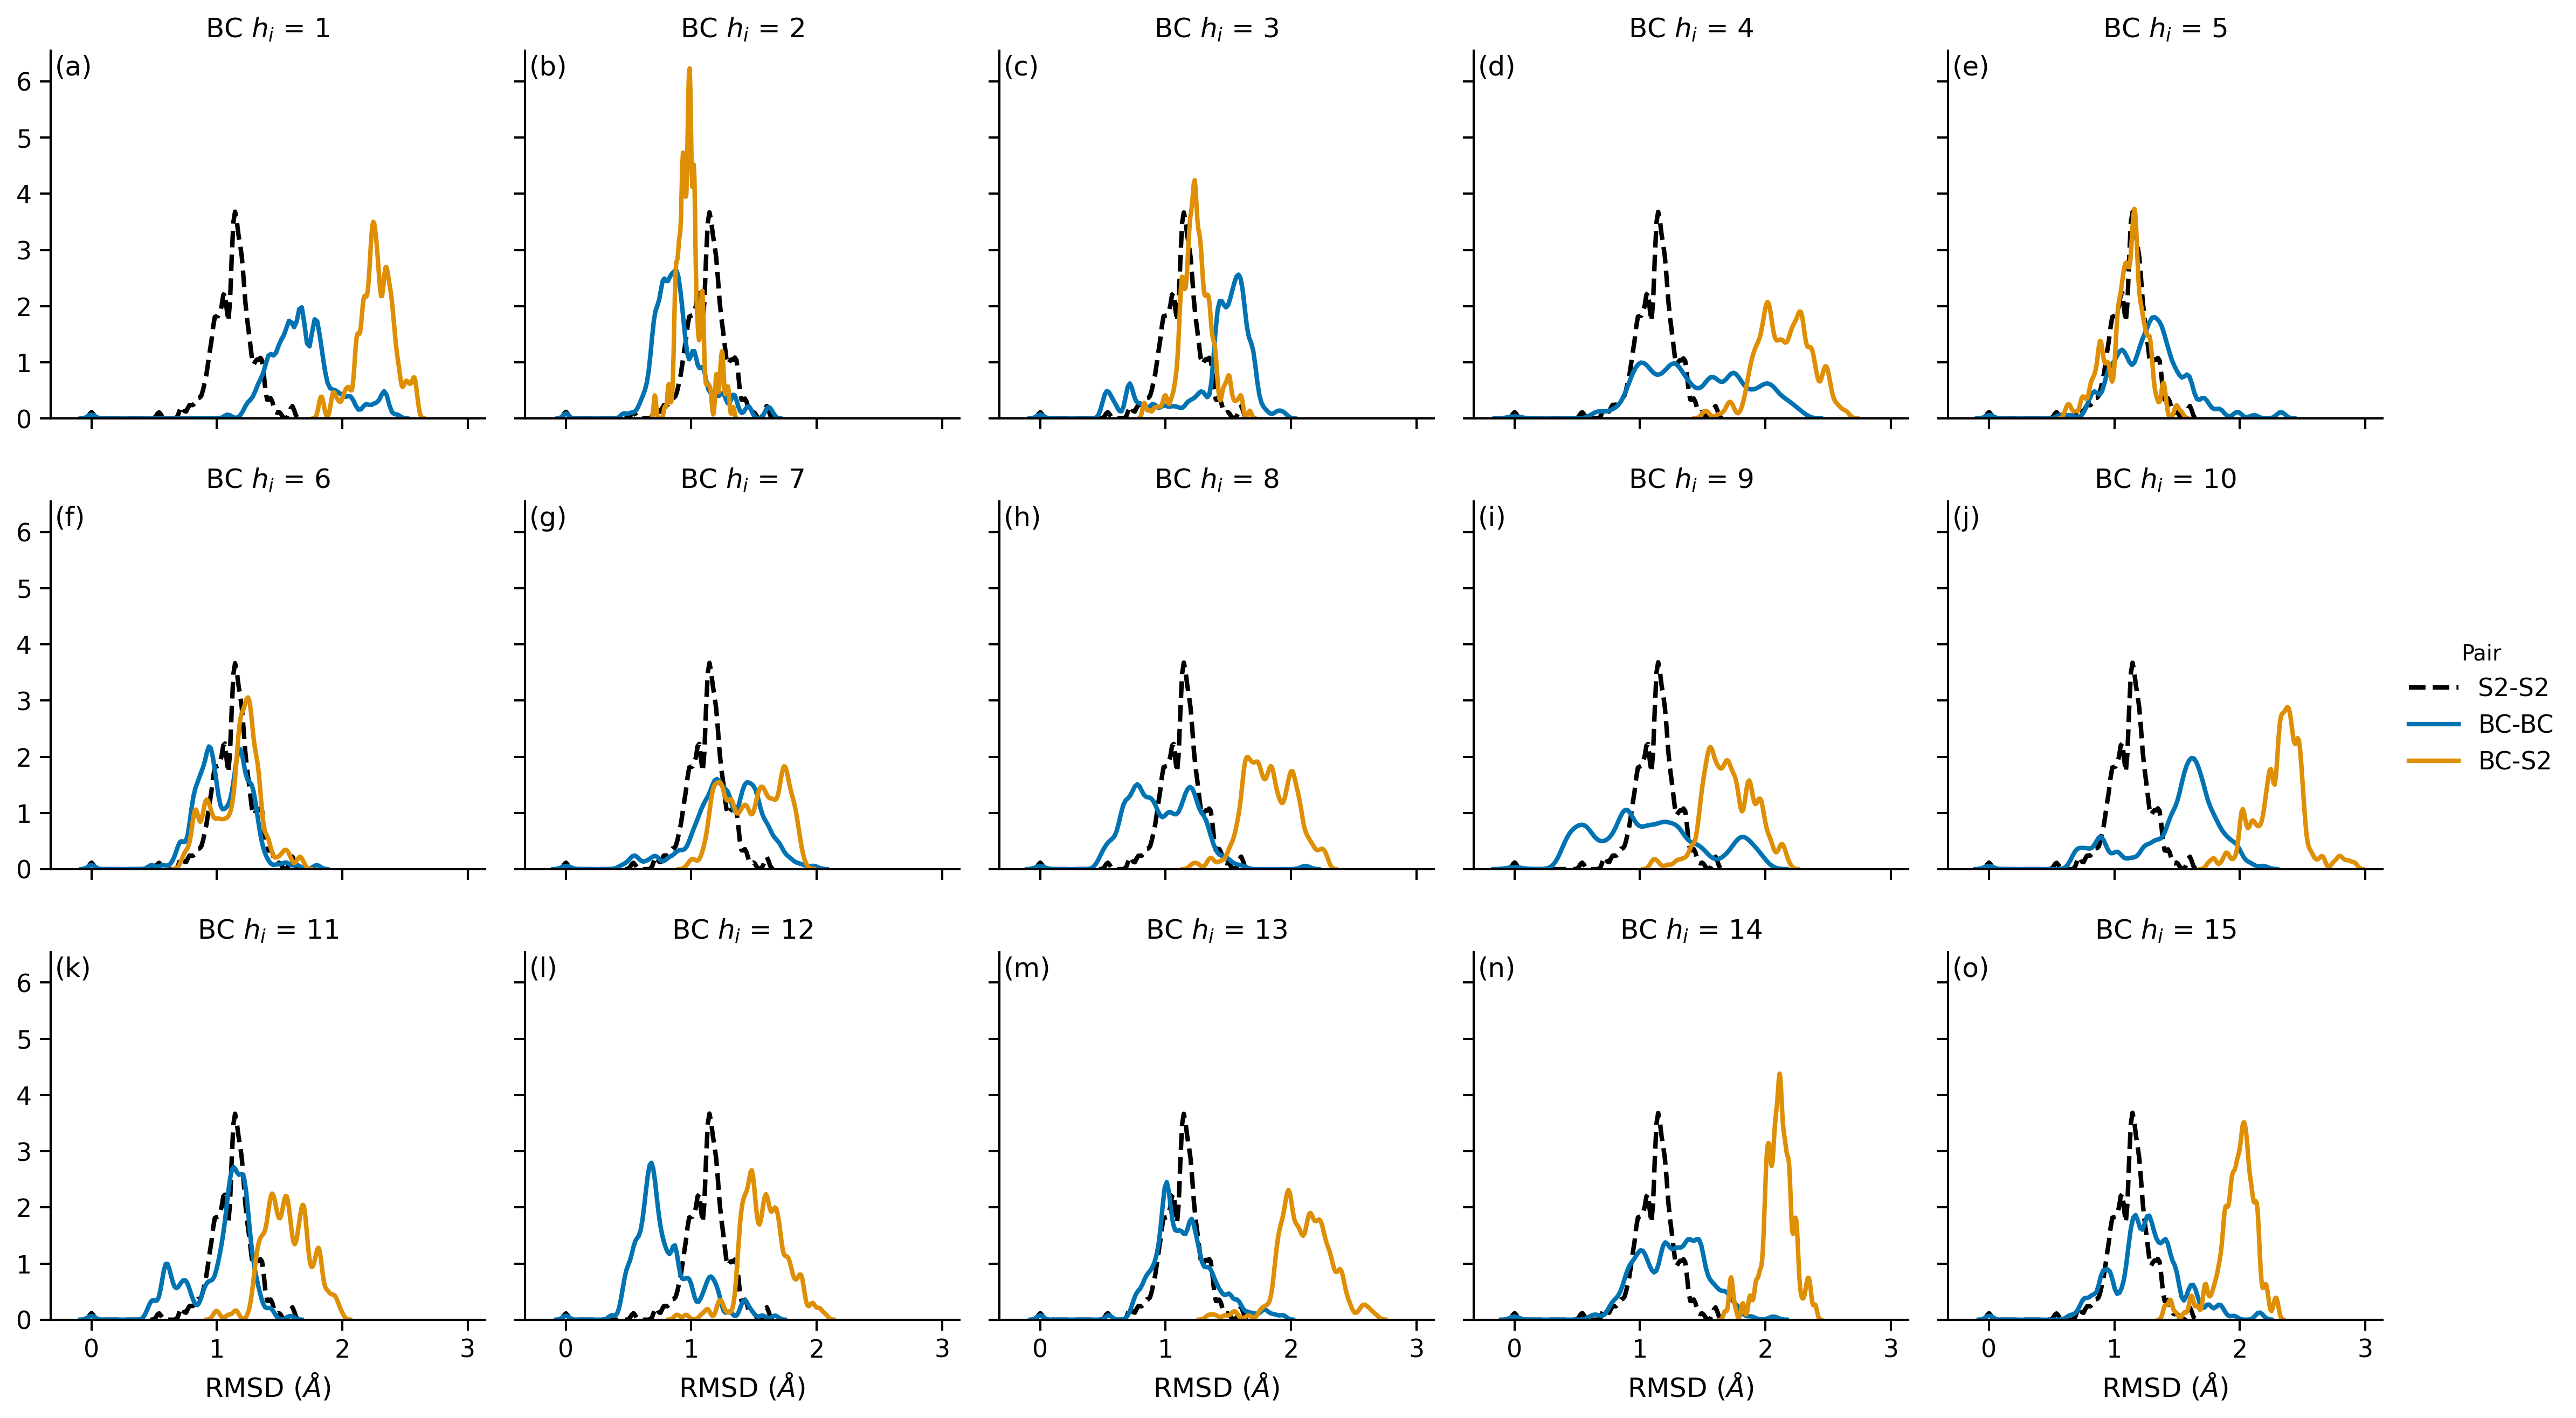
\includegraphics[width=0.8\textwidth]{chapters/aadh/figures/sensitivity_2_5_overlap.png}

\end{figure}




